\documentclass[preprint,11pt]{elsarticle}

\usepackage[T1]{fontenc}
\usepackage[utf8]{inputenc}
\usepackage[margin=0.95in]{geometry}
\usepackage{amsmath,amssymb,amsthm,mathtools}
\usepackage{bm}
\usepackage{booktabs}
\usepackage{multirow}
\usepackage{array}
\usepackage{graphicx}
\usepackage{subcaption}
\usepackage{xcolor}
\usepackage{hyperref}

\hypersetup{
  colorlinks=true,
  linkcolor=blue!60!black,
  citecolor=blue!60!black,
  urlcolor=blue!60!black
}

\journal{Computer Methods in Applied Mechanics and Engineering}

\newcommand{\R}{\mathbb{R}}
\newcommand{\C}{\mathbb{C}}
\newcommand{\T}{\mathbb{T}}
\newcommand{\Keff}{K_{\mathrm{eff}}}
\newcommand{\Keffij}[1]{K_{\mathrm{eff},#1}}
\newcommand{\Ceff}{\mathbb{C}^{\mathrm{eff}}}
\newcommand{\jump}[1]{[\![ #1 ]\!]}
\newcommand{\norm}[1]{\left\lVert #1 \right\rVert}
\newcommand{\abs}[1]{\left\lvert #1 \right\rvert}

\newtheorem{theorem}{Theorem}
\newtheorem{lemma}{Lemma}
\newtheorem{proposition}{Proposition}
\newtheorem{corollary}{Corollary}
\newtheorem{remark}{Remark}

\begin{document}

\begin{frontmatter}

\title{Boundary-Capacitance Neural Operators for High-Contrast Multiscale Homogenization}

\author[aff1]{Taiqian Liu}
\author[aff1,aff2]{Lijun Liu\corref{cor1}}
\ead{liulijun@xmu.edu.cn}
\author[aff3]{Chunhui Zhu}
\cortext[cor1]{Corresponding author.}

\address[aff1]{Department of Automation, School of Aerospace Engineering, Xiamen University, Xiamen 361005, China}
\address[aff2]{Shenzhen Research Institute of Xiamen University, Shenzhen 518000, China}
\address[aff3]{Institute of Electromagnetics and Acoustics, Xiamen University, Xiamen 361005, China}

\begin{abstract}
In high-contrast $\mathrm{FE}^2$ homogenization, standard $L^2$ field regression amplifies inclusion errors by $\Theta(\kappa)$ during constitutive averaging, while equipotential clamping removes that amplification only by discarding the $O(1)$ interior polarization flux ($-54\%$ underprediction on bridged inclusions at $\kappa=10^6$). Perfect-conductor clamping plus outer-boundary averaging becomes nearly exact at $\kappa\ge 10^4$, yet neither asymptotic extreme holds in the intermediate regime $\kappa\in[10,10^3]$ typical of engineering $\mathrm{FE}^2$ cells.

We resolve this gap with two discrete identities and the Boundary-Capacitance Neural Operator (BC-NO). For piecewise-constant media, the constant-coefficient Laplacian of the fluctuation is supported on the one-cell jump strip with contrast-bounded density $\sigma=h L_0(u-\ell)$. Shifting the classical virtual-work identity from the outer RVE boundary to the inclusion interface then recovers $\Keff$ and $\Ceff$ from matrix-side reactions alone ($\le 2\kappa_{\mathrm{mat}}$), giving contrast-invariant control on predicted fields. BC-NO combines $O(N^d\log N)$ constant-coefficient Green layers with normalized PDE residuals and connected-component capacitance pooling. Across fourteen benchmarks under a shared dipole readout, architectural OOD gains versus the strongest baseline per experiment are $1.0\times$--$4.1\times$ (readout alone often accounts for the rest); thermal and elastic $\mathrm{FE}^2$ plates reach $2.38\%$ flux and $0.61\%$ displacement error. Same-GPU 3D Jacobi-PCG speedups are $2.7\times$--$8.0\times$; same-CPU sparse LU is slower at $N=128$ ($0.86\times$) and faster only at $N\ge 256$.
\end{abstract}

\begin{keyword}
Multiscale homogenization \sep neural operators \sep high-contrast composites \sep boundary-capacitance reduction \sep $\mathrm{FE}^2$ \sep micro-CT microstructures
\end{keyword}

\end{frontmatter}

\section{Introduction}\label{sec:intro}

Computational homogenization—rooted in asymptotic multiscale analysis~\cite{bensoussan1978asymptotic,nemat1999micromechanics,milton2002theory} and realized numerically through FFT cell solvers~\cite{moulinec1998numerical,michel1999effective,schneider2021review} and coupled two-scale $\mathrm{FE}^2$ schemes~\cite{feyel2000fe2,miehe2002strain,geers2010multiscale,matous2017review}—provides the quantitative link between microscale heterogeneity and macroscopic continuum behavior in aerospace composites, porous geomaterials, and architected media. Because every macroscopic quadrature point or design iteration must query a representative volume element (RVE) involving $10^4$--$10^6$ degrees of freedom, accelerating the microscale constitutive map without losing physical fidelity remains a central bottleneck in multiscale mechanics.

To bypass repeated fine-scale solves, surrogate models span physics-structured reduced-order networks—such as Deep Material Networks~\cite{liu2019dmn}, recurrent history surrogates~\cite{ghavamian2019accelerating,mozaffar2019deep}, invariant Gaussian processes~\cite{fuhg2022physics}, and image-based CNNs~\cite{mianroodi2021teaching}—alongside neural operators including PCA-Net~\cite{bhattacharya2021model}, DeepONet~\cite{lu2021deeponet,lu2022fair}, FNO~\cite{li2021fno,kovachki2023neural}, U-NO~\cite{rahman2023uno}, FFNO~\cite{tran2023ffno}, CNO~\cite{raonic2023cno}, WNO~\cite{tripura2023wno}, MgNO~\cite{he2024mgno}, Transolver~\cite{wu2024transolver}, geometric and physics-informed variants~\cite{li2023geofno,li2023gino,li2024pino}, and micromechanical operators such as IFNO~\cite{you2022ifno}, composite stress-strain FNO~\cite{rashid2022learning}, U-FNO~\cite{nguyen2026ufno}, CGiNS~\cite{xing2025cgins}, and GMT~\cite{xing2026gmt}. Whether built directly in primal coordinates or coupled to Lippmann--Schwinger FFT solvers~\cite{eyre1999fast,brisard2010fft,zeman2010accelerating,monchiet2012polarization,kabel2014efficient,willot2015fourier}, direct field surrogates share an implicit assumption: that reducing the $L^2$ or energy-norm error of a predicted field $u_\theta$ guarantees an accurate homogenized tensor $\Keff$ or $\Ceff$ under standard flux or stress averaging.

At high engineering contrasts ($\kappa \in [10^2, 10^6]$), this assumption breaks down (Fig.~\ref{fig:failure_mech}). Writing the standard finite-volume readout as a linear functional $\Keff(u) = g \cdot u$, we show that the nodal sensitivity weights scale as $\abs{g_p} = \Theta(\kappa h)$ along phase interfaces with summed boundary $L^1$ sensitivity $\norm{g}_1 = \Theta(\kappa)$. Inside a conductive inclusion, the exact gradient is $O(1/\kappa)$, so correlated prediction errors of magnitude $O(\varepsilon)$ across an inclusion are amplified in worst-case or systematic-tilt scenarios to $\Theta(\kappa \varepsilon)$, producing errors of $10^3\%$--$10^5\%$ even when field $L^2$ error is modest. Conversely, clamping each inclusion to an equipotential constant eliminates $\Theta(\kappa)$ amplification but discards the $O(1)$ interior polarization flux, underpredicting $\Keff$ by $54.0\%$ on bridged topologies at $\kappa=10^6$. At $\kappa\ge 10^4$, the same clamp plus dipole averaging on the exact field is nearly exact ($0.99\%$ / $0.01\%$ on U-bridge at $\kappa=10^4$/$10^6$), so learning is not required in the perfect-conductor limit; at $\kappa\lesssim 10$, standard operators already suffice. The unresolved regime is the intermediate contrast band $\kappa\in[10,10^3]$ that dominates our $\mathrm{FE}^2$ plates ($\kappa\in[20,250]$, $E_1/E_0$ up to $10^3$), where neither asymptotic extreme holds. Existing ML homogenization frameworks either target moderate contrasts~\cite{mianroodi2021teaching,rashid2022learning,you2022ifno} or rely on iterative Krylov, multigrid V-cycle, or Lippmann--Schwinger outer corrections~\cite{nguyen2026ufno,xing2025cgins,xing2026gmt} to repair interface flux errors.

\begin{figure}[t]
  \centering
  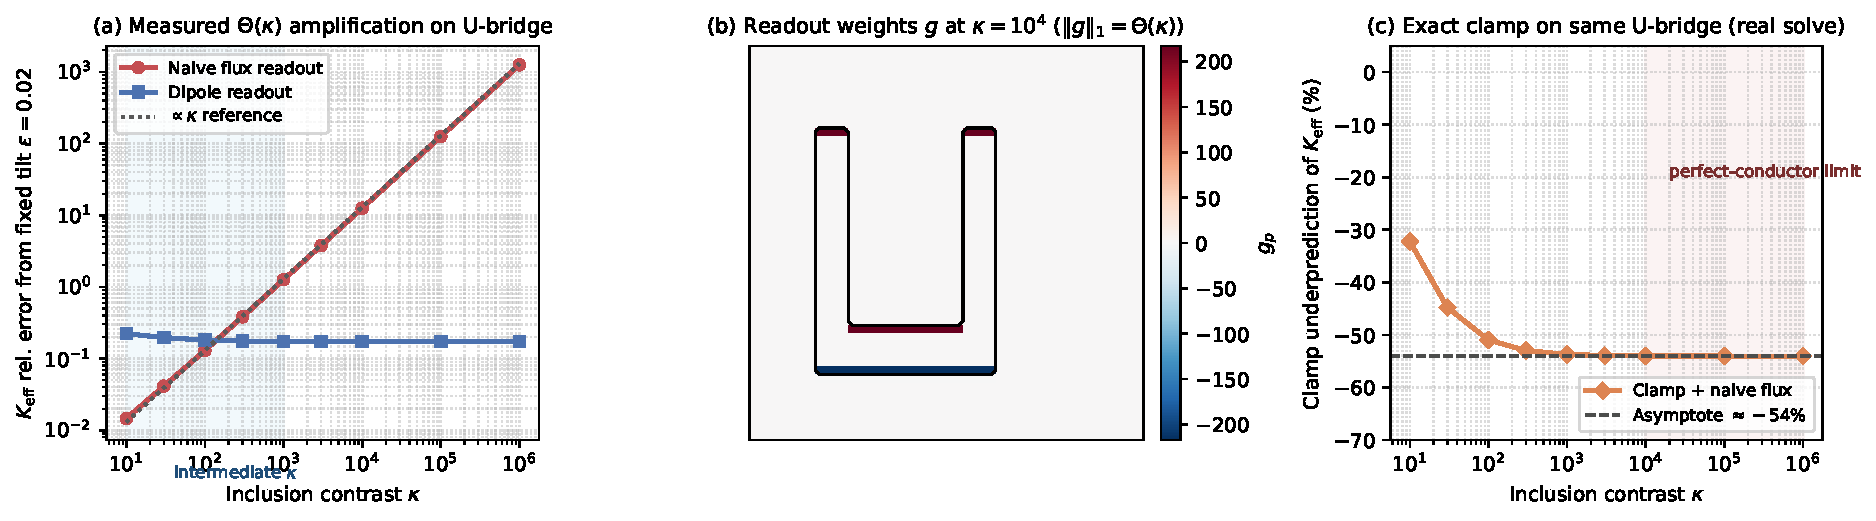
\includegraphics[width=\textwidth]{fig_empirical_mechanism.pdf}
  \caption{Empirical evidence of the failure mechanism on the same $48^2$ U-bridge used in Exp.~1 (exact harmonic-face solves; no schematic). (a) A fixed inclusion tilt of amplitude $\varepsilon=0.02$ yields naive $\Keff$ error that tracks $\propto\kappa$, while the dipole readout stays $O(1)$. (b) Nodal conservative-readout weights $g$ at $\kappa=10^4$ concentrate on the inclusion interface with $\norm{g}_1=\Theta(\kappa)$. (c) Equipotential clamping of the exact solution underpredicts $\Keff$ by $\approx 54\%$--$58\%$ as $\kappa\to\infty$, recovering the polarization-loss trade-off.}
  \label{fig:failure_mech}
\end{figure}

Eliminating this error amplification in a single-pass neural operator faces three coupled barriers. First, while high-contrast boundary integral equations (BIE)~\cite{greengard1994fast,cheng1998efficient,helsing2011integral} and multiscale finite element methods (MsFEM, HMM, domain decomposition, GMsFEM/CEM-GMsFEM, LOD, gamblets, and subspace-informed operators)~\cite{hou1997msfem,e2003hmm,chu2010new,galvis2010domain,efendiev2013gmsfem,malqvist2014localization,owhadi2017multigrid,chung2018cem,rudikov2026gmsfemno} achieve contrast-independent convergence via boundary layer potentials or oversampled spectral spaces, they still assemble and solve dense boundary or coarse-grid algebraic systems; meanwhile, standard neural networks regress bulk fields and suffer single-precision (\texttt{float32}) subtraction cancellation in PDE residuals at $\kappa = 10^6$. Second, disconnected conductive or stiff inclusions carry unknown floating potentials and rigid-body offsets coupled globally across narrow matrix gaps that local convolutional stencils cannot equilibrate. Third, achieving contrast-invariant inference on predicted (non-equilibrium) fields $\tilde u$ requires an algebraic reformulation whose error bound depends solely on bounded matrix-side conductances across Dirichlet, periodic, linear elastic, and nonlinear regimes, while preserving conservative flux transport on wall-to-wall percolating paths.

We address these barriers by embedding two discrete identities into the \textbf{Boundary-Capacitance Neural Operator (BC-NO)}. First, the constant-coefficient Laplacian source $\sigma = h L_0(u-\ell)$ vanishes outside the one-cell jump strip and is bounded by interface difference quotients independently of $\kappa$ (Lemma~\ref{thm:strip}), motivating an unrolled architecture with $O(N^d\log N)$ constant-coefficient Green operators ($\mathrm{DST}$-I, periodic $\mathrm{FFT}$, and Q1 Navier--Cauchy $\mathrm{FFT}$), dimensionless normalized PDE residuals ($w_{pq} \in [0,1]$), and vectorized connected-component capacitance pooling. Second, a discrete virtual-work boundary dipole identity yields contrast-invariant stability for arbitrary predicted fields (Theorem~\ref{thm:dipole} and Corollary~\ref{cor:stab}). Our contributions are:
\begin{enumerate}
  \item \textbf{Discrete identities and stability.} We characterize $\Theta(\kappa)$ sensitivity via $\abs{g_p} = \Theta(\kappa h)$ (Proposition~\ref{prop:amp}), prove one-cell strip localization of $\sigma = h L_0(u-\ell)$ (Lemma~\ref{thm:strip}), and establish a discrete virtual-work dipole identity with a contrast-independent stability bound on non-equilibrium predictions (Theorem~\ref{thm:dipole} and Corollary~\ref{cor:stab}). The novelty relative to standard $\mathrm{FE}^2$ reaction-force averaging~\cite{miehe2002strain,kouznetsova2001approach,geers2010multiscale} is relocating the identity from the outer RVE boundary to the inclusion interface, thereby removing $\kappa$ from the readout weights.
  \item \textbf{Boundary-Capacitance Neural Operator (BC-NO).} A compact ($57\mathrm{K}$--$93\mathrm{K}$ parameters) operator uniting $\mathrm{DST}$-I/$\mathrm{FFT}$ Green layers, bounded-weight residuals, component capacitance pooling, and percolation-aware adaptive dipole readouts across 2D/3D Dirichlet, 2D periodic, 2D vector elasticity, and nonlinear PDEs---targeting the intermediate-contrast regime where clamping asymptotics fail.
  \item \textbf{Fair comparison separating readout and architectural gains.} Under a shared dipole readout across fourteen studies (9 PDE baselines, \texttt{LS-FNO}, Willot CG-FFT, and non-collapsed CT/$32^3$/$64^3$ baselines), post-hoc dipole averaging accounts for most of the naive-to-dipole drop on external models; residual architectural OOD gains of BC-NO versus the strongest baseline \emph{per experiment} are $1.0\times$--$4.1\times$ (parity on nonlinear OOD with \texttt{MgNO}+dipole; $4.1\times$ at $1{,}000$ training samples on Exp.~2 OOD). Same-GPU Jacobi-PCG speedups are $2.7\times$--$8.0\times$; same-CPU sparse LU is $0.86\times$ at $N=128$.
  \item \textbf{Two-scale $\mathrm{FE}^2$ deployment with SPD projection.} With eigenvalue clipping at the Reuss lower bound $\lambda_{\min}\ge 1$, BC-NO reaches $2.36\%$ temperature and $2.38\%$ heat-flux error on a $16\times 16$ thermal plate (GPU inference vs.\ CPU sparse LU: $35.8\times$ wall-clock, a cross-hardware workflow comparison) and $0.61\%$/$0.59\%$ displacement/tip errors on a $20\times 10$ elastic cantilever (GPU vs.\ CPU FEM: $216\times$), versus $15.2\%$--$59.6\%$ flux error for dipole+SPD baselines.
\end{enumerate}

\section{Mathematical Formulation and Exact Structural Identities}\label{sec:theory}

\subsection{Discrete RVE Homogenization Setting}

Consider a heterogeneous RVE on the unit cell $\Omega = [0, 1]^d$ ($d \in \{2, 3\}$) discretized on a uniform Cartesian grid of $N^d$ nodes with spacing $h = 1/(N-1)$ (Dirichlet cell) or $h = 1/N$ (periodic torus $\T^d$). Let $\kappa(x) > 0$ denote the nodal conductivity field, partitioned into a matrix phase $\Omega_0$ ($\kappa = \kappa_0 = 1$, or smoothly varying $\kappa_{\mathrm{mat}}(x) = O(1)$) and a disjoint union of inclusions $I = \bigcup_{m=1}^M I_m$ with conductivity $\kappa_m \in (0, \infty)$. To ensure strict discrete flux conservation across sharp phase jumps, we adopt the node-centered harmonic-face finite-volume operator $A(\kappa)$: for every grid edge $(p, q)$ sharing a cell face, the effective face conductance is $k_{pq} = \frac{2 \kappa_p \kappa_q}{\kappa_p + \kappa_q}$, and the interior operator action is
\begin{equation}\label{eq:fvm}
  \big(A(\kappa) u\big)_p = \frac{1}{h^2} \sum_{q \in \mathcal{N}(p)} k_{pq} (u_p - u_q),
\end{equation}
where $\mathcal{N}(p)$ denotes the $2d$ axial neighbors of $p$. Under linear Dirichlet loading along axis $a \in \{1,\dots,d\}$, $u = \ell_a + v$ with $\ell_a(x) = x_a$ and $v|_{\partial \Omega} = 0$; under periodic loading, $v$ is $\T^d$-periodic with zero mean. The discrete solution satisfies $(A(\kappa) u)_p = 0$ at all free nodes. The homogenized effective conductivity column along load axis $a$ is defined by the spatial average of conservative interior face fluxes,
\begin{equation}\label{eq:keff_def}
  \Keffij{b,a}(u) = \frac{1}{\abs{\mathcal{F}_b^{\mathrm{int}}}} \sum_{(p,q) \in \mathcal{F}_b^{\mathrm{int}}} k_{pq} \frac{u_q - u_p}{h},
\end{equation}
where $\mathcal{F}_b^{\mathrm{int}}$ collects all interior-row axial faces oriented along direction $b$ ($q = p + h e_b$).

\subsection{Sensitivity Scaling, Strip Localization, and Virtual-Work Dipole Readout}

\begin{proposition}[Discrete sensitivity and worst-case $\Theta(\kappa)$ amplification]\label{prop:amp}
For any fixed conductivity field $\kappa$ on the $N\times N$ Dirichlet grid, there exists a unique sparse weight vector $g(\kappa) \in \R^{N\times N}$, supported exclusively on nodes adjacent to a conductivity jump or the outer boundary, such that for every grid function $\tilde u$ satisfying $\tilde u|_{\partial\Omega} = \ell_a|_{\partial\Omega}$,
\begin{equation}\label{eq:g_dot_u}
  \Keffij{a,a}(\tilde u) = \sum_{p} g_p(\kappa)\, \tilde u_p,
  \quad\text{hence}\quad
  \Keffij{a,a}(\tilde u) - \Keffij{a,a}(u) = \sum_{p} g_p(\kappa)\, (\tilde u_p - u_p).
\end{equation}
At any interior node $p$ located on the left or right boundary of a conductive inclusion $I_m$ of conductivity $\kappa \gg 1$—where one axial neighbor lies inside $I_m$ ($k_{pq} = \kappa$) and the opposite axial neighbor lies in the unit-conductivity matrix ($k_{pq'} = \frac{2\kappa}{\kappa+1} = 2 + O(\kappa^{-1})$)—the nodal sensitivity has magnitude $\abs{g_p} = \Theta(\kappa h)$ with opposite signs across the left and right faces of $I_m$, while $\sum_{p \in I_m} g_p = 0$ on every closed inclusion and $\norm{g}_1 = \sum_p \abs{g_p} = \Theta(\kappa)$. Consequently, $\abs{\Keffij{a,a}(\tilde u) - \Keffij{a,a}(u)} \le \norm{g}_1 \norm{\tilde u - u}_\infty = \Theta(\kappa \varepsilon)$ for $\norm{\tilde u - u}_\infty = \varepsilon$, attaining $\Theta(\kappa\varepsilon)$ in the worst case and under systematic errors correlated with $g$ (such as a linear tilt across $I_m$).
\end{proposition}

\begin{proof}
Because~\eqref{eq:keff_def} is linear in $u$, collecting coefficients of each nodal variable $u_p$ yields $g_p = \frac{1}{\abs{\mathcal{F}_a^{\mathrm{int}}} h}(k_{p-e_a,p} - k_{p,p+e_a})$ at interior rows (with missing boundary-side conductances set to zero). Since $\abs{\mathcal{F}_a^{\mathrm{int}}} = (N-2)(N-1) = \Theta(h^{-2})$, inside any constant-$\kappa$ phase $k_{p-e_a,p} = k_{p,p+e_a}$ so $g_p = 0$. At a left-boundary node of an inclusion ($\kappa_p = \kappa$, left neighbor $\kappa_{p-e_a}=1$, right neighbor $\kappa_{p+e_a}=\kappa$), $g_p = -\frac{\kappa - 2 + O(\kappa^{-1})}{(N-2)(N-1)h} = -\Theta(\kappa h)$; at the right-boundary node, the sign reverses to $+\Theta(\kappa h)$. Summing over the $\Theta(h^{-1})$ boundary nodes along the transverse height of $I_m$ yields $\norm{g}_1 = \Theta(\kappa)$, while summing over all nodes of any closed inclusion telescopes row-wise to $\sum_{p \in I_m} g_p = 0$. Thus a uniform constant shift on $I_m$ produces zero readout error, whereas a perturbation $e_p = \tilde u_p - u_p$ correlated with $\mathrm{sign}(g_p)$ yields $\abs{g\cdot e} = \Theta(\kappa\varepsilon)$.
\end{proof}

\begin{remark}[The equipotential-pinning trade-off]
Proposition~\ref{prop:amp} also clarifies why clamping each inclusion to a constant $\tilde u|_{I_m} \equiv c_m$ is inadequate: although $g \cdot c_m = 0$ removes $\Theta(\kappa)$ amplification, the exact interior potential satisfies $u|_{I_m} = c_m + w_m / \kappa + O(\kappa^{-2})$, so $g \cdot (w_m/\kappa) = O(1)$ supplies the interior polarization contribution. Clamping $\nabla \tilde u|_{I_m} = 0$ eliminates this $O(1)$ term in conservative flux readouts (measured as $-54.0\%$ underprediction on bridged inclusions at $\kappa=10^6$ in Section~\ref{sec:exp_hard}) and distorts the $O(1/\kappa)$ boundary values required by dipole readouts at moderate contrast ($88.8\%$ error on $N=128$ fibers).
\end{remark}

In boundary integral equation (BIE) and Lippmann--Schwinger polarization methods~\cite{greengard1994fast,cheng1998efficient,helsing2011integral,eyre1999fast,monchiet2012polarization}, piecewise-constant conductivity jumps induce an effective single-layer surface charge density supported on phase interfaces. Lemma~\ref{thm:strip} records the discrete algebraic counterpart on harmonic-face grids.

\begin{lemma}[Boundary-strip support and $\kappa$-uniform density bound]\label{thm:strip}
Let $L_0 = A(1)$ denote the constant-coefficient ($\kappa \equiv 1$) discrete Laplacian, and let $\partial I$ denote the one-cell jump strip consisting of interior cells adjacent to at least one face with $\kappa_p \neq \kappa_q$. For any piecewise-constant conductivity field $\kappa$ and exact solution $u = \ell_a + v$ satisfying $(A(\kappa)u)_p = 0$ at free nodes, the discrete surface density $\sigma_p := h (L_0 v)_p$ satisfies
\begin{equation}\label{eq:sigma_exact}
  \sigma_p = \frac{1}{\kappa_p} \sum_{q \in \mathcal{N}(p)} (\kappa_p - k_{pq}) \frac{u_p - u_q}{h} \qquad \forall p \notin \partial\Omega.
\end{equation}
Consequently: (i) $\sigma_p = 0$ for every $p \notin \partial I \cup \partial\Omega$; (ii) $\abs{\kappa_p - k_{pq}} / \kappa_p < 1$ for all $\kappa_p, \kappa_q \in (0, \infty)$; and (iii) $v = G_0(\sigma / h)$ with $G_0 = L_0^{-1}$.
\end{lemma}

\begin{proof}
Because $\ell_a$ is discrete affine-harmonic ($L_0 \ell_a = 0$), $(L_0 v)_p = (L_0 u)_p$. Subtracting $0 = \frac{1}{\kappa_p}(A(\kappa)u)_p = \frac{1}{\kappa_p h^2}\sum_{q\in\mathcal{N}(p)} k_{pq}(u_p - u_q)$ from $(L_0 u)_p = \frac{1}{h^2}\sum_{q\in\mathcal{N}(p)} (u_p - u_q)$ and multiplying by $h$ yields~\eqref{eq:sigma_exact} identically. If $p \notin \partial I$, all neighbors share $\kappa_q = \kappa_p$, so $k_{pq} = \kappa_p$ and $\sigma_p = 0$. On the unit-conductivity matrix side ($\kappa_p = 1$), $k_{pq} = \frac{2\kappa_q}{1+\kappa_q} \in (0, 2)$ implies $\abs{1 - k_{pq}} < 1$; on the inclusion side ($\kappa_p = \kappa > 0$), because $k_{pq} = \frac{2\kappa}{\kappa+1}$, for $\kappa \ge 1$ we have $0 \le \frac{\kappa - k_{pq}}{\kappa} = \frac{\kappa - 1}{\kappa + 1} < 1$, while for $0 < \kappa < 1$ we have $k_{pq} \in (\kappa, 2\kappa)$ so $\abs{\frac{\kappa - k_{pq}}{\kappa}} = \frac{1-\kappa}{1+\kappa} < 1$. Hence $\abs{\sigma_p} \le \sum_{q\in\mathcal{N}(p)} \abs{u_p - u_q}/h$ uniformly across all contrasts $\kappa \in (0, \infty)$.
\end{proof}

Averaging reaction forces on the \emph{outer} RVE boundary is standard in $\mathrm{FE}^2$~\cite{miehe2002strain,kouznetsova2001approach,geers2010multiscale} and follows from Hill's lemma~\cite{nemat1999micromechanics,milton2002theory}. Theorem~\ref{thm:dipole} relocates that virtual-work identity to the \emph{inclusion interface} on harmonic-face finite-volume and Q1 grids, so that the readout weights involve only matrix-side conductances; Corollary~\ref{cor:stab} then bounds the error for non-equilibrium predictions $\tilde u$.

\begin{theorem}[Discrete virtual-work boundary dipole identity]\label{thm:dipole}
Let $\mathcal{I}_{\mathrm{np}} \subset I$ be the union of all interior (non-percolating) conductive components, and partition faces $\mathcal{F}_b^{\mathrm{int}}$ into interior-inclusion faces $\mathcal{F}_b^{\mathrm{inc}} = \{(p,q) : p,q \in \mathcal{I}_{\mathrm{np}}\}$ and exterior/interface faces $\mathcal{F}_b^{\mathrm{ext}} = \mathcal{F}_b^{\mathrm{int}} \setminus \mathcal{F}_b^{\mathrm{inc}}$. For any exact solution $u$ of $(A(\kappa)u)_p = 0$ on $\mathcal{I}_{\mathrm{np}}$,
\begin{equation}\label{eq:dipole_id}
  \Keffij{b,a}(u) = \frac{1}{\abs{\mathcal{F}_b^{\mathrm{int}}}} \sum_{(p,q) \in \mathcal{F}_b^{\mathrm{ext}}} k_{pq} \frac{u_q - u_p}{h}
  \;-\; \frac{1}{\abs{\mathcal{F}_b^{\mathrm{int}}}} \sum_{p \in \mathcal{I}_{\mathrm{np}}} x_{b,p}\, \big(A_{\mathrm{ext}}(\kappa) u\big)_p,
\end{equation}
where $\big(A_{\mathrm{ext}}(\kappa) u\big)_p := \frac{1}{h^2} \sum_{q \in \mathcal{N}(p)\setminus \mathcal{I}_{\mathrm{np}}} k_{pq}(u_p - u_q)$ sums exclusively over matrix-side interface neighbors with bounded conductances $k_{pq} = \frac{2\kappa_p\kappa_q}{\kappa_p+\kappa_q} \le 2\kappa_{\mathrm{mat}} = O(1)$. Under periodic boundary conditions on $\T^d$, the same identity holds with $x_{b,p}$ replaced by the torus-wrapped displacement $\mathrm{wrap}(x_{b,p} - \bar x_{b,m})$ relative to each component's circular centroid $\bar x_m$, because $\sum_{p\in I_m} (A_{\mathrm{ext}} u)_p = 0$. In 2D Q1 finite-element linear elasticity with stiff elements $\mathcal{I}_{\mathrm{np}}$ ($E_{\mathrm{inc}} \gg 1$), let $\partial\mathcal{I}_{\mathrm{np}}$ denote the set of nodes shared by at least one inclusion element in $\mathcal{I}_{\mathrm{np}}$ and one matrix element outside $\mathcal{I}_{\mathrm{np}}$, and let $\bm{f}^{\mathrm{mat}}_p$ denote the nodal internal force assembled exclusively over matrix elements ($E_{\mathrm{mat}} = O(1)$) so that exact equilibrium reads $\bm{f}^{\mathrm{inc}}_p + \bm{f}^{\mathrm{mat}}_p = \bm{0}$ at every $p \in \partial\mathcal{I}_{\mathrm{np}}$. Virtual work with $\bm{w}^{(b)}(x) = \mathrm{wrap}(x - \bar x_m) \otimes e_b$ yields
\begin{equation}\label{eq:elas_dipole}
  \bar\sigma_{bc} = \sum_{e \notin \mathcal{I}_{\mathrm{np}}} \sigma_{bc}^{(e)}\, h^2 - \frac{1}{2}\sum_{p \in \partial \mathcal{I}_{\mathrm{np}}} \Big( \mathrm{wrap}(x_{b,p}-\bar x_{b,m}) f^{\mathrm{mat}}_{c,p} + \mathrm{wrap}(x_{c,p}-\bar x_{c,m}) f^{\mathrm{mat}}_{b,p} \Big).
\end{equation}
\end{theorem}

\begin{proof}
For every $p \in \mathcal{I}_{\mathrm{np}}$, discrete equilibrium $(A(\kappa) u)_p = 0$ decomposes into internal and matrix-interface parts: $(A_{\mathrm{int}}(\kappa) u)_p + (A_{\mathrm{ext}}(\kappa) u)_p = 0$. Testing $(A_{\mathrm{int}}(\kappa) u)_p$ against $x_{b,p}$ and summing over $p \in \mathcal{I}_{\mathrm{np}}$ yields, by discrete summation by parts,
\[
  \sum_{p \in \mathcal{I}_{\mathrm{np}}} x_{b,p} (A_{\mathrm{int}}(\kappa) u)_p
  = \frac{1}{h^2} \sum_{(p,q) \in \mathcal{F}_b^{\mathrm{inc}}} k_{pq}(x_{b,p} - x_{b,q})(u_p - u_q)
  = \frac{1}{h} \sum_{(p,q) \in \mathcal{F}_b^{\mathrm{inc}}} k_{pq}(u_q - u_p),
\]
because transverse edges $(p, q)$ perpendicular to $e_b$ satisfy $x_{b,p} = x_{b,q}$ and vanish identically, while axial edges satisfy $x_{b,q} - x_{b,p} = h$. Substituting $(A_{\mathrm{int}} u)_p = -(A_{\mathrm{ext}} u)_p$ directly recovers~\eqref{eq:dipole_id}. Because $A_{\mathrm{ext}}$ touches only interface faces between $I_m$ and $\Omega_{\mathrm{mat}}$, $k_{pq} \le 2\kappa_{\mathrm{mat}}$ is bounded independently of $\kappa_m$ and of whether $\kappa_{\mathrm{mat}}$ is linear or nonlinear ($\kappa(x, u)$). Under periodic BCs, equilibrium gives $\sum_{p \in I_m} (A_{\mathrm{ext}} u)_p = 0$, rendering the sum invariant to the periodic branch choice via $\bar x_{b,m}$. In Q1 linear elasticity, global equilibrium $\bm{f}^{\mathrm{inc}}_p + \bm{f}^{\mathrm{mat}}_p = \bm{0}$ gives
\[
  \sum_{e\in\mathcal{I}_{\mathrm{np}}} \int_e \bm{\sigma} : \nabla \bm{w}\, \mathrm{d}A = \sum_p \bm{w}_p \cdot \bm{f}^{\mathrm{inc}}_p = -\sum_p \bm{w}_p \cdot \bm{f}^{\mathrm{mat}}_p,
\]
which yields~\eqref{eq:elas_dipole} upon symmetrization.
\end{proof}

Theorem~\ref{thm:dipole} is an identity for exact solutions $u$; a surrogate $\tilde u$ need not satisfy $(A(\kappa)\tilde u)_p = 0$ inside $\mathcal{I}_{\mathrm{np}}$. The following corollary justifies~\eqref{eq:dipole_id}--\eqref{eq:elas_dipole} as a neural readout for \textbf{arbitrary non-equilibrium fields $\tilde u$}.

\begin{corollary}[Contrast-invariant readout stability on predicted fields]\label{cor:stab}
Define the right-hand side of~\eqref{eq:dipole_id} as a linear functional $\Keffij{b,a}^{\mathrm{dip}}(\tilde u)$ acting on any grid field $\tilde u$. Because $\Keffij{b,a}^{\mathrm{dip}}(\tilde u)$ accesses $\kappa$ exclusively through conductances $k_{pq}$ on $\mathcal{F}_b^{\mathrm{ext}}$ and on interface edges leaving $\mathcal{I}_{\mathrm{np}}$—all of which satisfy $k_{pq} \le 2\max_{\Omega_{\mathrm{mat}}}\kappa_{\mathrm{mat}}$—the readout satisfies
\begin{equation}\label{eq:dip_stab}
  \abs{\Keffij{b,a}^{\mathrm{dip}}(\tilde u) - \Keffij{b,a}(u)}
  = \abs{\Keffij{b,a}^{\mathrm{dip}}(\tilde u - u)}
  \le C(\kappa_{\mathrm{mat}}, \mathcal{I}_{\mathrm{np}})\,\norm{\tilde u - u}_{1,\mathrm{ext}},
\end{equation}
where $\norm{e}_{1,\mathrm{ext}} := \max_{(p,q)\in \mathcal{F}_b^{\mathrm{ext}} \cup \partial\mathcal{I}_{\mathrm{np}}^{\mathrm{ext}}} \frac{\abs{e_q - e_p}}{h}$ measures \emph{interface and matrix-side difference quotients}, not the global field max-norm. For geometries with bounded interface measure $\abs{\partial\mathcal{I}_{\mathrm{np}}^{\mathrm{ext}}} h^{d-1} \le \mathrm{Per}(\mathcal{I}_{\mathrm{np}}) < \infty$, the constant $C(\kappa_{\mathrm{mat}}, \mathcal{I}_{\mathrm{np}}) = O(\max_{\Omega_{\mathrm{mat}}}\kappa_{\mathrm{mat}} \cdot (1 + \mathrm{Per}(\mathcal{I}_{\mathrm{np}})))$ is independent of all non-percolating inclusion conductivities $\kappa_m \in (0, \infty)$ and of $h$. Under Dirichlet loading the virtual-work weights use the raw coordinate $x_b$; a floating potential offset $\delta$ on an inclusion therefore couples through the dipole term at order $\delta/h$, transferring sensitivity from $\kappa$ to interface gradients and mesh scale. This is precisely why connected-component capacitance pooling is required: it constrains floating potentials before readout. For~\eqref{eq:elas_dipole}, the same matrix-side argument yields an analogous formal bound with $C(E_{\mathrm{mat}}, \mathcal{I}_{\mathrm{np}})$ independent of $E_{\mathrm{inc}}$; a fully expanded elasticity proof is left for future work, and we rely on the discrete virtual-work derivation above together with numerical identity checks.
\end{corollary}

\begin{proof}
By Theorem~\ref{thm:dipole}, $\Keffij{b,a}(u) = \Keffij{b,a}^{\mathrm{dip}}(u)$ for the exact solution $u$. Linearity gives $\Keffij{b,a}^{\mathrm{dip}}(\tilde u) - \Keffij{b,a}(u) = \Keffij{b,a}^{\mathrm{dip}}(e)$ with $e = \tilde u - u$. Each face $(p,q) \in \mathcal{F}_b^{\mathrm{ext}}$ contributes $\abs{k_{pq}}/\abs{\mathcal{F}_b^{\mathrm{int}}} \cdot \abs{e_q-e_p}/h$, whose sum over $\mathcal{F}_b^{\mathrm{ext}}$ is bounded by $2\max_{\Omega_{\mathrm{mat}}}\kappa_{\mathrm{mat}}\norm{e}_{1,\mathrm{ext}}$. Since $\abs{x_{b,p}} \le 1$, each matrix-crossing interface edge $(p,q) \in \partial\mathcal{I}_{\mathrm{np}}^{\mathrm{ext}}$ contributes at most $\frac{k_{pq}}{\abs{\mathcal{F}_b^{\mathrm{int}}} h^2}\abs{e_p - e_q} = \frac{k_{pq}}{\abs{\mathcal{F}_b^{\mathrm{int}}} h}\frac{\abs{e_p - e_q}}{h}$. Because $\abs{\mathcal{F}_b^{\mathrm{int}}} = \Theta(h^{-d})$ and $\abs{\partial\mathcal{I}_{\mathrm{np}}^{\mathrm{ext}}} \le \mathrm{Per}(\mathcal{I}_{\mathrm{np}}) h^{-(d-1)}$, summing over $\partial\mathcal{I}_{\mathrm{np}}^{\mathrm{ext}}$ introduces the factor $\frac{\abs{\partial\mathcal{I}_{\mathrm{np}}^{\mathrm{ext}}}}{\abs{\mathcal{F}_b^{\mathrm{int}}} h} = O(\mathrm{Per}(\mathcal{I}_{\mathrm{np}}))$ independent of $h$. As every appearing conductance satisfies $k_{pq} \le 2\max_{\Omega_{\mathrm{mat}}} \kappa_{\mathrm{mat}}$, the stability constant is independent of $\kappa_m$.
\end{proof}

We verify Theorem~\ref{thm:dipole} numerically in double precision across all regimes at $\kappa = 10^4$ ($E_1/E_0 = 10^3$ for elasticity): the discrepancy between~\eqref{eq:dipole_id}--\eqref{eq:elas_dipole} and the direct volume average is $1.38\times 10^{-11}$ (2D Dirichlet), $6.93\times 10^{-14}$ (2D periodic with boundary-wrapping ellipse), $5.30\times 10^{-12}$ (3D Dirichlet), $7.76\times 10^{-13}$ (2D Q1 elasticity), and $2.29\times 10^{-11}$ (2D nonlinear conduction $-\nabla\cdot(\kappa_0(x)(1+3u^2)\nabla u)=0$ on a continuous log-normal matrix with star inclusions).

\section{Boundary-Capacitance Neural Operator (BC-NO)}\label{sec:method}

Guided by Lemma~\ref{thm:strip}, Theorem~\ref{thm:dipole}, and Corollary~\ref{cor:stab}, BC-NO represents the predicted solution as $u_\theta = \ell_a + G_0(\sigma_\theta / h)$ through $T$ unrolled boundary-capacitance updates ($T=4$ in 2D, $T=3$ in 3D), initialized at $\sigma^{(0)} = 0$ and $u^{(0)} = \ell_a$, as illustrated in Fig.~\ref{fig:bcno_arch}. Constant-coefficient Green solves ($G_0$), standard convolutions, and \texttt{scatter\_add} follow FFT-homogenization~\cite{moulinec1998numerical} and standard deep-learning primitives; the $\kappa$-bounded weight residual~\eqref{eq:r_flux}, connected-component capacitance pooling~\eqref{eq:cap_pool}, one-cell jump-strip source update~\eqref{eq:sigma_upd}, and percolation-aware adaptive dipole readout are the components introduced here.

\begin{figure}[t]
  \centering
  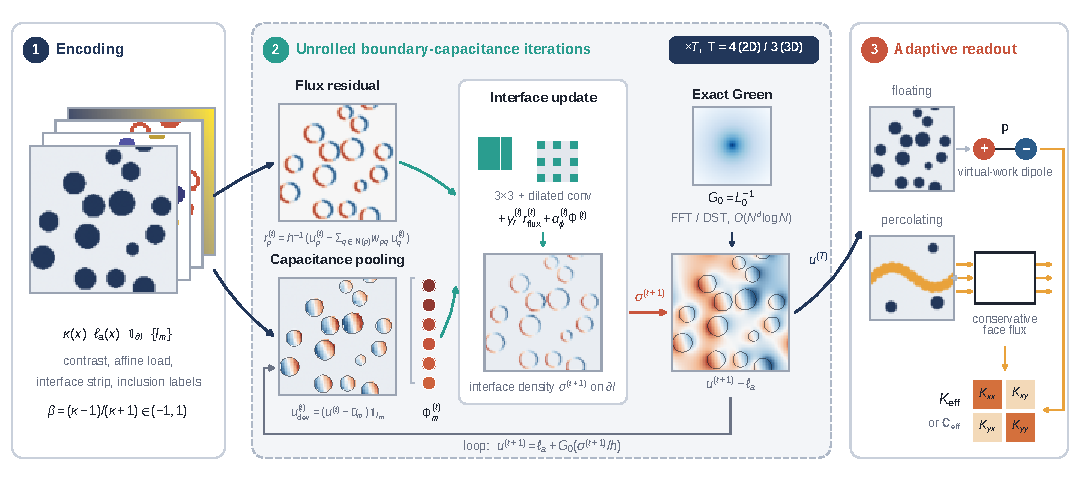
\includegraphics[width=\textwidth]{fig_bcno_architecture_v2.pdf}
  \caption{End-to-end architecture of the Boundary-Capacitance Neural Operator (BC-NO). Stage~1 encodes the conductivity field into bounded features, normalized neighbor weights $w_{pq}\in[0,1]$, and connected-component labels $\{I_m\}$. Stage~2 iterates $T$ unrolled updates combining dimensionless PDE residuals $r_{p}^{(t)}$, vectorized capacitance pooling $(u_{\mathrm{dev}}^{(t)}, \Phi_m^{(t)})$, a compact local network $\mathcal{B}_\theta^{(t)}$ masked to the one-cell jump strip $\partial I$, and an $O(N^d \log N)$ constant-coefficient Green solve $G_0 = L_0^{-1}$. Stage~3 applies a percolation-aware adaptive readout (virtual-work dipole for floating inclusions, conservative face flux for percolating paths) to recover $\Keff$ or $\Ceff$.}
  \label{fig:bcno_arch}
\end{figure}

\subsection{Exact Constant-Coefficient Green Layers}
For Dirichlet RVEs on $[0,1]^d$ ($d=2,3$), the interior discrete Laplacian $L_0$ is diagonalized by the orthonormal Discrete Sine Transform ($\mathrm{DST}$-I), realized differentiably via odd-symmetric reflection and \texttt{torch.fft.fft}:
\[
  G_0(s) = \mathcal{S}^{-1}\!\left(\frac{\mathcal{S}(s)}{\lambda^{\mathrm{DST}}}\right),
  \qquad
  \lambda^{\mathrm{DST}}_{k_1,\dots,k_d} = \sum_{r=1}^d \frac{2 - 2\cos(\pi k_r / (N-1))}{h^2}.
\]
For 2D periodic RVEs, $G_0^{\mathrm{per}}$ uses 2D \texttt{rfft2}/\texttt{irfft2} with the zero mode zeroed. For 2D Q1 linear elasticity, $G_0^{\mathrm{elas}}$ inverts the $2\times 2$ block periodic Q1 Navier--Cauchy symbol $M(\bm{\xi}) \in \C^{2\times 2}$ in \texttt{rfft2} space (verified to $6.88\times 10^{-15}$). Every Green step runs in $O(N^d \log N)$ time without dense linear solves.

\subsection{Contrast-Bounded Residuals}
Evaluating $A(\kappa) u$ in single precision (\texttt{float32}) at $\kappa = 10^6$ causes subtraction cancellation: interior differences $u_p - u_q \sim 10^{-7}$ multiplied by $\kappa = 10^6$ produce $O(10^{-1})$ rounding noise that corrupts component sums. We therefore compute normalized PDE residuals with dimensionless neighbor weights $w_{pq} = k_{pq} / \sum_{q'} k_{pq'} \in [0, 1]$,
\begin{equation}\label{eq:r_flux}
  r_{\mathrm{flux}, p}(u) = \frac{1}{h}\!\left(u_p - \sum_{q \in \mathcal{N}(p)} w_{pq}(\kappa)\, u_q\right),
\end{equation}
so no $O(\kappa)$ quantity enters the forward pass. Conductivities are encoded via the bounded reflection factor $\beta = \frac{\kappa - 1}{\kappa + 1} \in (-1, 1)$ and scaled log-contrast $\frac{1}{10}\log\kappa$.

\subsection{Vectorized Connected-Component Capacitance Pooling}
For each floating conductive component $I_m \subset \Omega$ ($\kappa > 1.5$, excluding components touching $\partial\Omega$ in Dirichlet cells or wall-to-wall percolating components in periodic cells), we compute two size-invariant global descriptors in $O(N^d)$ time via vectorized \texttt{scatter\_add}:
\begin{equation}\label{eq:cap_pool}
  u_{\mathrm{dev}, p} = (u_p - \bar u_m)\mathbf{1}_{p \in I_m},
  \qquad
  \Phi_m = \frac{\sum_{p \in I_m} (A_{\mathrm{ext}}(\kappa) u)_p}{\abs{\partial I_m}},
\end{equation}
where $\bar u_m = \mathrm{mean}_{I_m}(u)$ tracks equipotential violation and $\Phi_m$ measures net exterior flux imbalance per unit boundary length using only matrix-side interface conductances ($\le 2$, avoiding internal cancellation). In 2D Q1 elasticity, the same pooling computes the rigid-translation deviation and net matrix reaction force $(F_{x,m}, F_{y,m})$ per inclusion.

\subsection{Unrolled Interface Update and Adaptive Readout}
At step $t \in \{0,\dots,T-1\}$, a compact convolutional block $\mathcal{B}_\theta^{(t)}$ (3--4 layers of $3\times 3$ and dilated $3\times 3$ convolutions, width $32$ in 2D or $16$--$20$ in 3D, $57\mathrm{K}$--$93\mathrm{K}$ parameters total) takes the $14$-channel stacked input
\[
  \Big[\beta,\; \tfrac{1}{10}\log\kappa,\; \mathbf{1}_{\partial I},\; \mathbf{1}_{\mathrm{cond}},\; \mathbf{1}_{\mathrm{insul}},\; \mathbf{1}_{\mathrm{float}},\; \ell_a,\; \ell_\perp,\; d_{\partial\Omega},\; u^{(t)},\; r_{\mathrm{flux}}^{(t)},\; 10 u_{\mathrm{dev}}^{(t)},\; \Phi^{(t)},\; \sigma^{(t)}\Big],
\]
where $\mathbf{1}_{\partial I}$ marks the one-cell jump strip, $\mathbf{1}_{\mathrm{cond}} = \mathbf{1}_{\{\kappa > 1.5\}}$ and $\mathbf{1}_{\mathrm{insul}} = \mathbf{1}_{\{\kappa < 0.67\}}$ indicate conductive and insulating inclusions, $\mathbf{1}_{\mathrm{float}}$ marks floating conductive components $I_m$, $\ell_\perp$ is the orthogonal coordinate ($x_2$ for $a=1$, $x_1$ for $a=2$), and $d_{\partial\Omega}(x) = 2\min_{k\in\{1,\dots,d\}}\min(x_k, 1-x_k) \in [0, 1]$ is the normalized distance to $\partial\Omega$. The update evolves as
\begin{align}\label{eq:sigma_upd}
  \sigma^{(t+1)} &= \sigma^{(t)} + \Big(\mathcal{B}_\theta^{(t)}(\cdot) + \gamma_r^{(t)}\, r_{\mathrm{flux}}^{(t)} + \alpha_\phi^{(t)}\, \Phi^{(t)}\Big)\mathbf{1}_{\partial I}, \nonumber\\
  u^{(t+1)} &= \ell_a + G_0\!\left(\frac{\sigma^{(t+1)}}{h}\right),
\end{align}
with learnable physics skip weights initialized at $\gamma_r^{(t)} = -2.0$. On problems with continuously varying matrices or nonlinear conductivities $\kappa(x,u)$ (Section~\ref{sec:exp_fe2_nl}), $\mathbf{1}_{\partial I}$ is relaxed to the interior domain and $\kappa(x, u^{(t)})$ is re-evaluated at each step $t$. During inference, $\Keff$ is evaluated via~\eqref{eq:dipole_id}, where wall-to-wall percolating components along either axis are excluded from $\mathcal{I}_{\mathrm{np}}$ so that percolating laminates retain conservative face-flux accuracy while non-percolating inclusions remain contrast-invariant.

\subsection{Training Objective}
Models are trained using a dimensionless composite loss balancing relative fluctuation $L^2$, relative $\Keff$ error via~\eqref{eq:dipole_id}, and surface density MSE on $\partial I$:
\begin{equation}
  \mathcal{L} = \mathbb{E}\!\left[\frac{\norm{v_\theta - v}_{2}}{\max(\norm{v}_{2}, 10^{-2})} + 0.25\,\frac{\abs{\Keff^{\mathrm{dip}}(u_\theta) - \Keff}}{\max(\abs{\Keff}, 0.1)} + 0.25\,\frac{\norm{(\sigma_\theta - \sigma)\mathbf{1}_{\partial I}}_2^2}{\abs{\partial I}}\right],
\end{equation}
where $\sigma = h L_0 v$ is computed directly from the ground-truth fluctuation without extra labels.

\section{Experimental Setup, Datasets, and Protocols}\label{sec:setup}

\subsection{Datasets and ID/OOD Splits}
All reference solutions are computed in double precision (\texttt{float64}) via sparse LU (\texttt{scipy.\allowbreak sparse.\allowbreak linalg.\allowbreak spsolve}) in 2D and preconditioned conjugate gradient / sparse LU in 3D, with conservative face-flux ground-truth tensors $\Keff$ satisfying Onsager symmetry. Fourteen benchmarks span five problem classes:
\begin{itemize}
  \item \textbf{Hard topologies (Exp.~1 \& Exp.~4b):} $48^2$ geometries (Exp.~1: 8 training shapes at $\kappa \in \{20, 10^2, 10^3, 10^4\}$ tested zero-shot on unseen \texttt{wall}, \texttt{center}, \texttt{bridge}, and \texttt{Lhold} up to $\kappa = 10^6$) and $N=128$ multi-family benchmarks (Exp.~4b: \texttt{hard\_bridge\_1e6} with near-wall boxes, U-bridges, and L-shapes trained at $\kappa \in [20, 10^4]$ and tested at $\kappa = 10^6$; \texttt{wavy\_laminate} with sinusoidal bands trained at $\kappa \in [10, 80]$ and tested up to $\kappa = 500$; $64$ train / $32$ ID / $32$ OOD samples each).
  \item \textbf{Fiber composites \& cross-resolution (Exp.~2, 3, 5, 5b, 11):} \texttt{fiber\_columns} ($N=128$) places $3$--$6\times 3$--$6$ jittered elliptic fibers with $25\%$ insulating ($\kappa < 1$) and $75\%$ conductive ($\kappa > 1$) realizations: Exp.~2 uses $128$ train / $64$ ID ($\kappa \in [10, 80]$ or reciprocals, $\mathrm{vf} \in [0.25, 0.55]$) and $64$ OOD ($\kappa \in [100, 300]$, $\mathrm{vf} \in [0.40, 0.65]$, frequent percolating clusters). Exp.~5/5b evaluates cross-resolution models (trained with zero $N=256$ data) at $N=64$ and $N=256$. Exp.~11 scales training to $1{,}000$ samples ($200$ ID) and evaluates on both the Exp.~2 OOD split and a harder high-percolation OOD split ($\kappa \in [100, 400]$, $\mathrm{vf} \in [0.45, 0.72]$).
  \item \textbf{Real micro-CT volumes (Exp.~6, 8, 12):} \texttt{real\_ct\_32} ($32^2$ multi-mineral locked test slices normalized by median $\kappa$, including homogeneous zero-fluctuation slices) and segmented Ruhr sandstone micro-CT patches ($\kappa_{\mathrm{mineral}} = 10^3$, $\kappa_{\mathrm{pore}} = 1$) extracted from disjoint $z$-slabs at $128^2$ ($48$ train / $24$ test), $32^3$ ($72$ train / $36$ test), and $64^3$ ($108$ train / $36$ test), alongside synthetic $32^3$/$64^3$ ellipsoids and fibers ($\kappa \in [10, 80]$ ID $\to [200, 10^3]$ OOD).
  \item \textbf{Periodic, linear elastic, and nonlinear PDEs (Exp.~7, 9, 13):} 2D PBC ($N=64$, wrapped ellipses, $\kappa \in [10, 80]$ ID $\to [100, 300]$ OOD); 2D periodic Q1 linear elasticity ($N=48$, $E_1/E_0 \in [10, 200]$ ID $\to [500, 10^3]$ OOD, 3 strain modes); nonlinear conduction $-\nabla\cdot(\kappa_0(x)(1+3u^2)\nabla u)=0$ on continuous log-normal matrices with sharp non-convex star inclusions ($\kappa_{\mathrm{star}} \in [20, 500]$ ID $\to [10^3, 10^4]$ OOD, $400$ train / $100$ ID / $100$ OOD).
  \item \textbf{Two-scale $\mathrm{FE}^2$ structures (Exp.~10 \& Exp.~14):} A $16\times 16$ Q1 thermal plate ($256$ graded $128^2$ RVEs, $\kappa(x) \in [20, 250]$, $\mathrm{vf} \in [0.28, 0.62]$) and a $20\times 10$ Q1 linear-elasticity composite cantilever with a central circular cutout ($184$ active $64^2$ periodic RVEs $\times 3$ strain modes, $E_1/E_0$ graded from $30$ at the clamped root to $1{,}000$ OOD around the hole; models trained solely on $E_1/E_0 \in [10, 200]$).
\end{itemize}

\subsection{Evaluation Metrics}
For paired RVE loading along all $d$ coordinate axes, we report: (i) the \textbf{paired tensor Frobenius relative error} $\norm{\tilde K - \Keff}_F / \norm{\Keff}_F$ ($\Keff$ Err), (ii) the \textbf{diagonal relative error} $\abs{\tilde K_{aa} - \Keffij{aa}} / \abs{\Keffij{aa}}$ (Diag), (iii) the \textbf{fluctuation relative $L^2$ error} $\norm{v_\theta - v}_2 / \norm{v}_2$ (over non-trivial samples with $\norm{v}_2 > 10^{-4}$), and (iv) the \textbf{energy-norm error} $\big(\int_\Omega \kappa \abs{\nabla(u_\theta - u)}^2 / \int_\Omega \kappa \abs{\nabla u}^2\big)^{1/2}$. Constitutive admissibility is audited via Onsager symmetry $\abs{\tilde K_{12}-\tilde K_{21}}/\norm{\tilde K}_F$, positive-definiteness rate ($\lambda_{\min}(\tfrac{1}{2}(\tilde K+\tilde K^\top)) > 0$), and Voigt--Reuss compliance.

\subsection{Baselines, Tuning Protocol, and Hardware Timing Parity}
We benchmark BC-NO against nine general PDE architectures—\textbf{FNO2d/3d}~\cite{li2021fno}, \textbf{ResUNet}, \textbf{U-NO}~\cite{rahman2023uno}, \textbf{FFNO2d}~\cite{tran2023ffno}, \textbf{CNO2d}~\cite{raonic2023cno}, \textbf{MgNO2d}~\cite{he2024mgno}, \textbf{Transolver2d}~\cite{wu2024transolver} ($32$ physical slices), and energy-norm variants \textbf{MgNO2d+Energy} and \textbf{ResUNet+Energy}~\cite{xing2025cgins}—plus two homogenization-specific references: a classical \textbf{Willot rotated-grid CG-FFT solver}~\cite{willot2015fourier,zeman2010accelerating} ($\mathrm{tol}=10^{-6}$, geometric-mean reference $\kappa_0 = \sqrt{\kappa_{\min}\kappa_{\max}}$) and an unrolled \textbf{Lippmann--Schwinger FNO (\texttt{LS-FNO})} motivated by~\cite{nguyen2026ufno}, iterating $u^{(t+1)} = \ell_a + \alpha^{(t)} G_0(\mathcal{N}_\theta^{(t)}(\kappa, \nabla u^{(t)})) + (1-\alpha^{(t)}) u^{(t)}$. All external models receive identical bounded contrast features $[\beta, \tfrac{1}{10}\log\kappa, \ell_a, \ell_\perp, d_{\partial\Omega}]$ and hard outer Dirichlet enforcement. To separate readout gains from architectural gains fairly, \textbf{our primary comparisons evaluate every model using the identical dipole readout~\eqref{eq:dipole_id}}, while also reporting conservative naive readouts.

For BC-NO, AdamW with cosine annealing uses $\mathrm{lr}=3\times 10^{-3}$ ($\mathrm{weight\_decay}=10^{-5}$, $100$ epochs in Exp.~2, $80$ in Exp.~5b/7/9/10/14, $75$ in Exp.~3/4b, $50$--$60$ in Exp.~11--13). External baselines use the same optimizer schedule with a grid over $\mathrm{lr}\in\{10^{-4},3\times 10^{-4},10^{-3},2\times 10^{-3},3\times 10^{-3}\}$, $\mathrm{weight\_decay}\in\{0,10^{-5}\}$, and modes $\in\{8,12,16\}$ (FNO/FFNO/UNO) or channel widths matching published defaults (ResUNet, MgNO, CNO, Transolver); we select the lowest validation $\Keff$ dipole error per model. Energy-named baselines (\texttt{MgNO2d+Energy}, \texttt{ResUNet+Energy}) are trained with energy-norm field losses and evaluated under the same dipole protocol as all other models. Separately, the variational energy identity $K_{aa}=\langle u^{(a)}, A(\kappa)u^{(a)}\rangle$ is applied as a readout on identical predicted fields: on exact solutions, naive, dipole, and energy readouts agree; on learned fields, dipole yields the lowest OOD tensor error (BC-NO $0.088$ dipole vs.\ $0.939$ energy; FNO $0.49$ vs.\ $7.59$). Under $128$ training samples the strongest all-dipole OOD error among baselines is $0.403$ (Exp.~2); with $1{,}000$ samples it falls to $0.336$ while BC-NO reaches $0.082$ (Exp.~11). On a regenerated fiber subset with identical schedules, BC-NO validation dipole error decreases from $0.172$ to $0.150$ over $60$ epochs, while FNO/ResUNet/MgNO remain between $0.44$ and $0.70$. In initial 2D CT and 3D runs, output heads initialized with $\mathrm{std}=10^{-3}$ collapsed to zero fluctuation ($\mathrm{Fluct}\,L^2 = 1.000$) under relative-$L^2$ training with zero-fluctuation slices; we resolved this by re-initializing baseline heads with standard Kaiming scaling, normalizing losses by training target RMS ($\mathrm{v}_{\mathrm{rms}}$) with $0.5\,\mathrm{MSE}_{\mathrm{norm}} + 0.5\,\mathrm{Rel}L^2$ ($\mathrm{weight\_decay}=0$), and retuning $\mathrm{lr}$ as above for $80$--$100$ epochs ($50$ at $64^3$). Timing protocol reports both residual-driven Willot CG-FFT / Jacobi-PCG at $\mathrm{tol}=10^{-6}$ and matched-accuracy early-stop of Willot when $\Keff$ error relative to the FVM reference reaches $30\%$, $10\%$, and $5\%$ ($3$, $5$, and $7$ GPU iterations; $\approx 11$--$13\text{ ms}$/sample). The $1\%$ band is not attained: the rotated-grid FFT and harmonic-face FVM discretizations differ by about $3\%$--$4\%$ even at convergence. Same-CPU sparse LU uses a 4-thread Apple M3; $\mathrm{FE}^2$ GPU-vs-CPU wall-clock ratios are reported as end-to-end workflow times.

\section{Results and Analysis}\label{sec:results}

\subsection{Contrast Amplification, Equipotential Clamping, and Hard Topologies (Exp.~1 \& Exp.~4b)}\label{sec:exp_hard}

\begin{figure}[t]
  \centering
  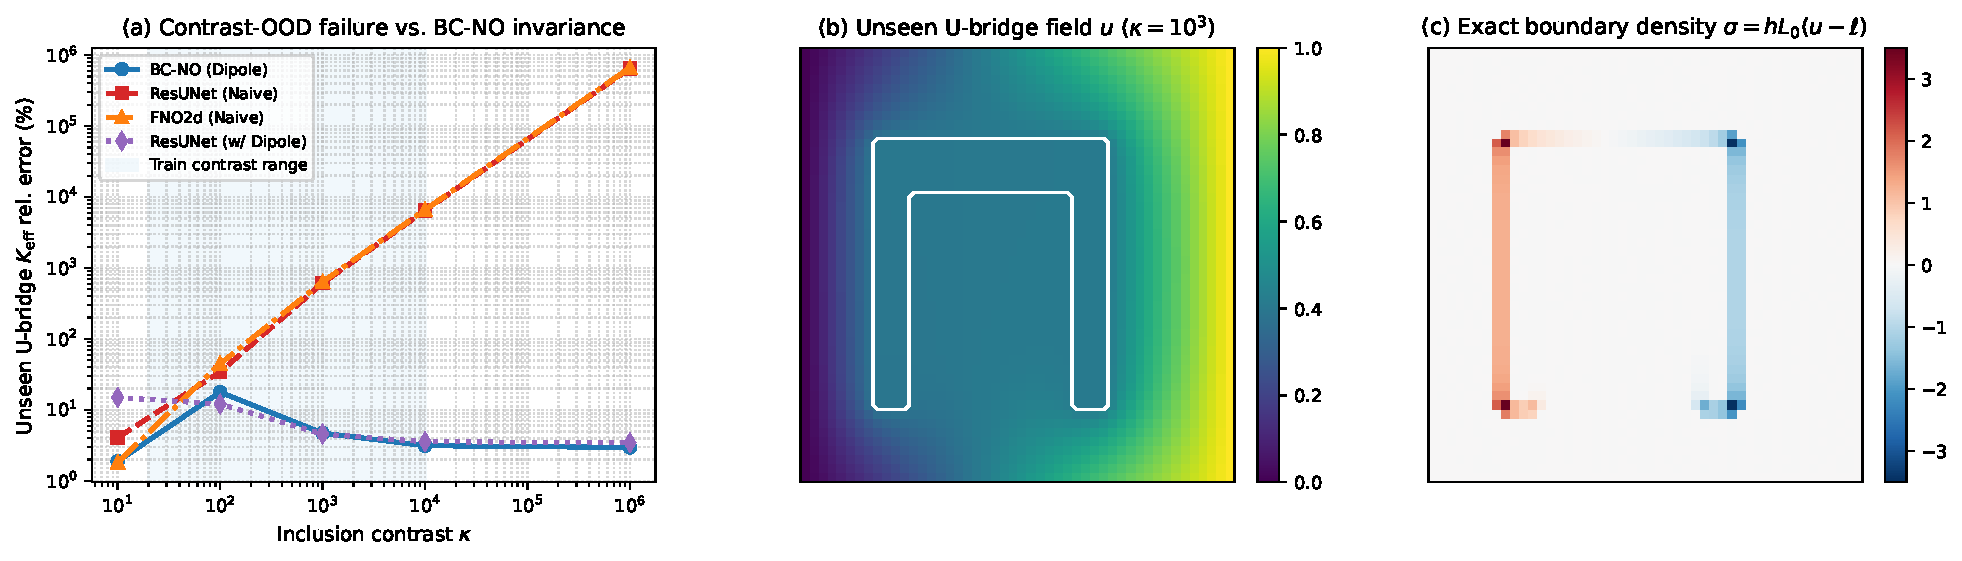
\includegraphics[width=\textwidth]{fig1_mechanism_contrast_ood.pdf}
  \caption{Mechanism validation on $48\times 48$ hard geometries. (a) Zero-shot contrast extrapolation ($\kappa \in [10, 10^6]$) on an unseen U-bridge: naive readouts amplify error linearly with $\kappa$ ($6.6\times 10^5\%$ at $\kappa=10^6$), whereas BC-NO remains bounded ($2.96\%$). (b) Exact potential $u$ on the U-bridge ($\kappa = 10^3$). (c) Exact boundary density $\sigma = h L_0(u-\ell)$ confirming one-cell jump-strip support.}
  \label{fig:mechanism}
\end{figure}

\begin{table}[t]
\centering
\caption{Exp.~1 ($48^2$ unseen geometries, trained at $\kappa \in [20, 10^4]$, tested up to $\kappa=10^6$ OOD, incl.\ equipotential-clamped reference) and Exp.~4b ($N=128$ multi-family benchmarks, 3 seeds, mean $\pm$ std). Each $\Keff$ cell reports Dipole / Naive relative error for that model; missing Naive entries are marked ---.}
\label{tab:hard}
\resizebox{\textwidth}{!}{%
\begin{tabular}{@{}llcccccc@{}}
\toprule
Benchmark & Model & \multicolumn{2}{c}{$\kappa = 10^2$} & \multicolumn{2}{c}{$\kappa = 10^4$} & \multicolumn{2}{c}{$\kappa = 10^6$ (OOD)} \\
\cmidrule(lr){3-4}\cmidrule(lr){5-6}\cmidrule(lr){7-8}
 & & $\Keff$ (Dip / Naive) & Field $L^2$ & $\Keff$ (Dip / Naive) & Field $L^2$ & $\Keff$ (Dip / Naive) & Field $L^2$ \\
\midrule
\multirow{3}{*}{$48^2$ Wall}
 & BC-NO & \textbf{5.76\%} / 13.7\% & \textbf{0.024} & \textbf{4.93\%} / 412\% & \textbf{0.050} & \textbf{4.88\%} / $4.3\times 10^4\%$ & 0.051 \\
 & ResUNet & 7.36\% / --- & 0.036 & 11.4\% / 121\% & 0.032 & 10.3\% / $1.2\times 10^4\%$ & \textbf{0.032} \\
 & FNO2d & 20.6\% / --- & 0.075 & --- / --- & 0.077 & 8.22\% / $1.6\times 10^5\%$ & 0.077 \\
\midrule
\multirow{3}{*}{$48^2$ Center}
 & BC-NO & \textbf{0.62\%} / 1.46\% & \textbf{0.005} & \textbf{0.58\%} / 302\% & \textbf{0.005} & \textbf{0.57\%} / $3.0\times 10^4\%$ & \textbf{0.005} \\
 & ResUNet & 7.47\% / --- & 0.011 & 6.23\% / --- & 0.010 & 6.10\% / $2.9\times 10^4\%$ & 0.010 \\
 & FNO2d & 3.92\% / --- & 0.033 & 1.24\% / --- & 0.035 & 1.19\% / $3.1\times 10^4\%$ & 0.035 \\
\midrule
\multirow{4}{*}{$48^2$ U-bridge}
 & BC-NO & 17.8\% / 18.2\% & \textbf{0.114} & \textbf{3.14\%} / 68.7\% & \textbf{0.064} & \textbf{2.96\%} / $4.1\times 10^5\%$ & \textbf{0.063} \\
 & ResUNet & 34.4\% / 34.4\% & 0.162 & 64.9\% / 6439\% & 0.219 & 3.45\% / $6.5\times 10^5\%$ & 0.220 \\
 & FNO2d & 44.8\% / 44.8\% & 0.160 & 58.6\% / 6615\% & 0.213 & 57.9\% / $6.6\times 10^5\%$ & 0.213 \\
 & Equipot.\ Clamped & 93.7\% / $-51.0\%$ & --- & 0.99\% / $-54.0\%$ & --- & 0.01\% / $-54.0\%$ & --- \\
\midrule
\multirow{4}{*}{$48^2$ L-hold}
 & BC-NO & \textbf{3.58\%} / 4.21\% & \textbf{0.022} & \textbf{2.37\%} / 521\% & \textbf{0.029} & \textbf{2.36\%} / $5.2\times 10^5\%$ & \textbf{0.029} \\
 & ResUNet & 67.9\% / 67.9\% & 0.086 & 29.8\% / 5988\% & 0.090 & 29.2\% / $6.0\times 10^5\%$ & 0.090 \\
 & FNO2d & 88.9\% / 88.9\% & 0.085 & 8.95\% / 9730\% & 0.092 & 8.79\% / $9.7\times 10^5\%$ & 0.092 \\
 & Equipot.\ Clamped & 25.7\% / $-28.2\%$ & --- & 0.27\% / $-30.0\%$ & --- & 0.00\% / $-30.0\%$ & --- \\
\midrule
$128^2$ Hard Bridge & BC-NO (3 seeds) & \multicolumn{2}{c}{ID Frob: $0.008\pm 0.002$ (Diag: $0.006$)} & \multicolumn{2}{c}{OOD $\kappa=10^6$:} & \textbf{0.024}$\pm$0.002 (Diag: \textbf{0.018}) / $2234.0$ & \textbf{0.061}$\pm$0.005 \\
$128^2$ Wavy Lam. & BC-NO (3 seeds) & \multicolumn{2}{c}{ID Frob: $0.034\pm 0.001$ (Diag: $0.066$)} & \multicolumn{2}{c}{OOD $\kappa\le 500$:} & \textbf{0.036}$\pm$0.001 (Diag: \textbf{0.158}) / $0.200$ & \textbf{0.157}$\pm$0.003 \\
\bottomrule
\end{tabular}}
\end{table}

Figure~\ref{fig:mechanism} and Table~\ref{tab:hard} verify Proposition~\ref{prop:amp} and Corollary~\ref{cor:stab} across all four $48^2$ geometries. Under naive conservative readout, \texttt{ResUNet} and \texttt{FNO2d} reach field $L^2$ errors of $0.99\%$ (\texttt{center}) to $22.0\%$ (\texttt{bridge}), yet incur $1.2\times 10^4\%$--$9.7\times 10^5\%$ errors in naive $\Keff$ at $\kappa=10^6$. Clamping the exact solution to an equipotential constant inside inclusions eliminates naive $\Theta(\kappa)$ blowup, but underpredicts $\Keff$ by $-54.0\%$ on \texttt{bridge} and $-30.0\%$ on \texttt{Lhold}. The same clamp plus dipole readout on the exact field is nearly exact at extreme contrast ($0.99\%$ / $0.01\%$ on U-bridge at $\kappa=10^4$/$10^6$), confirming that learning is unnecessary in the perfect-conductor limit. Applying dipole readout~\eqref{eq:dipole_id} post hoc to external baselines reduces their $\kappa=10^6$ naive errors into the few-percent to tens-of-percent range (e.g., \texttt{ResUNet} $3.45\%$ on \texttt{bridge}, $29.2\%$ on \texttt{Lhold}; \texttt{FNO2d} $57.9\%$ on \texttt{bridge}). Relative to the strongest dipole baseline per geometry, BC-NO improves by $1.2\times$ on U-bridge ($2.96\%$ vs.\ ResUNet $3.45\%$), $2.1\times$ on center ($0.57\%$ vs.\ FNO2d $1.19\%$), $1.7\times$ on wall ($4.88\%$ vs.\ FNO2d $8.22\%$), and $3.7\times$ on L-hold ($2.36\%$ vs.\ FNO2d $8.79\%$). Scaled to $N=128$ (Exp.~4b; $64$ train / $32$ ID / $32$ OOD), BC-NO achieves $0.008\pm 0.002$ ID and $0.024\pm 0.002$ OOD Frobenius error on \texttt{hard\_bridge\_1e6}, and $0.034\pm 0.001$ ID / $0.036\pm 0.001$ OOD on \texttt{wavy\_laminate}.

\subsection{Primary Fiber Benchmark at Scale (Exp.~11) and 128-Sample Reference (Exp.~2)}\label{sec:exp_fiber}

\begin{figure}[t]
  \centering
  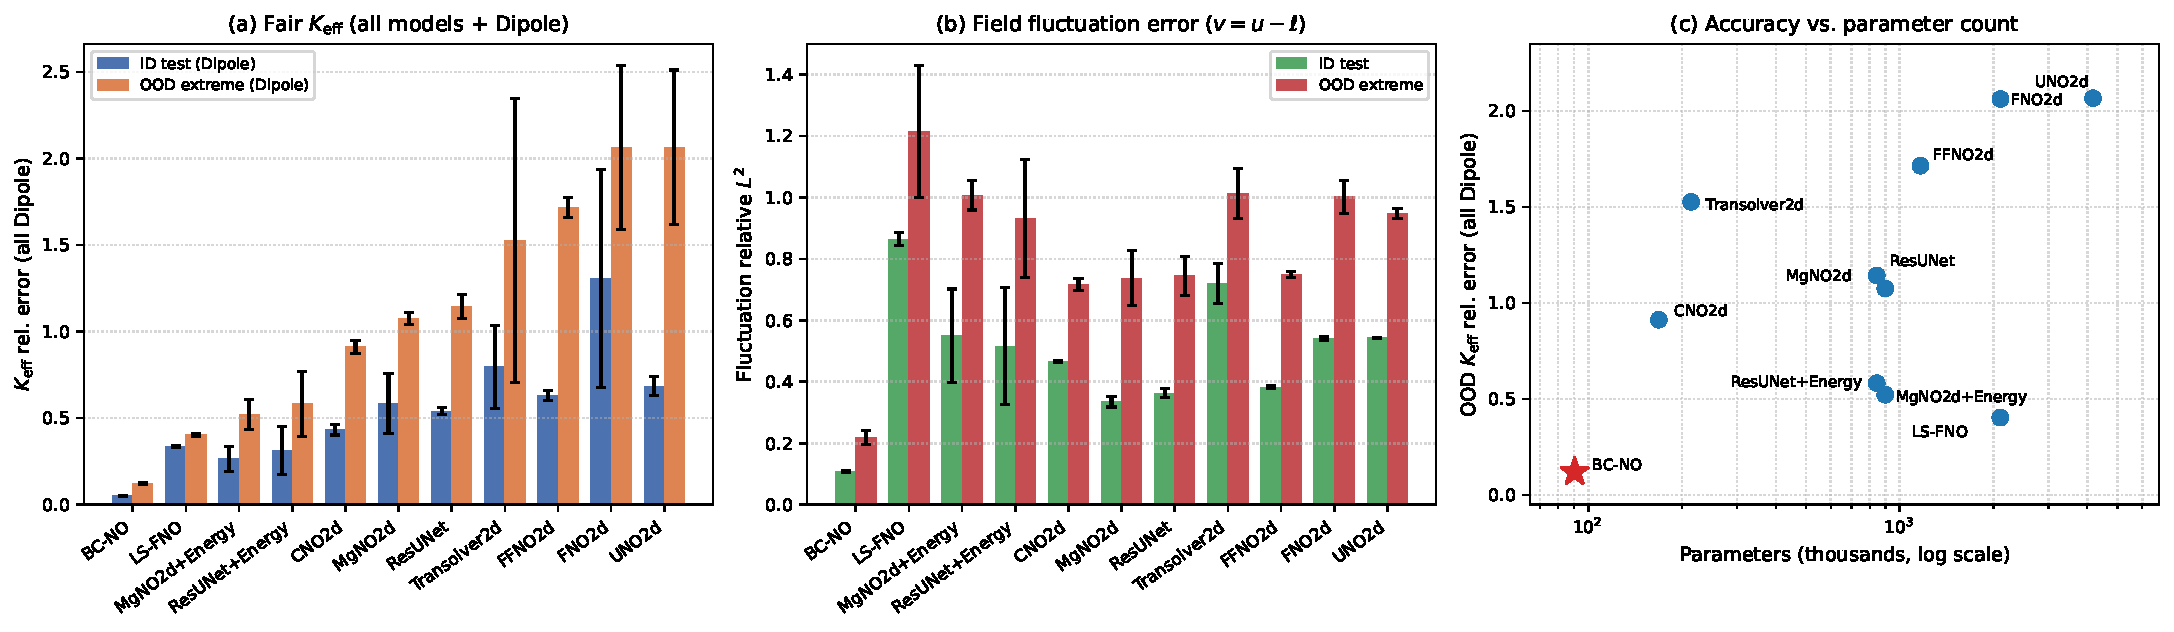
\includegraphics[width=\textwidth]{fig2_fiber_n128_benchmark.pdf}
  \caption{$N=128$ \texttt{fiber\_columns} benchmark (3 seeds, mean $\pm$ std) evaluated fairly with all models using the dipole readout~\eqref{eq:dipole_id}, including the homogenization-specific \texttt{LS-FNO}. (a) Fair $\Keff$ relative error. (b) Field fluctuation $L^2$ error. (c) Accuracy versus parameter count Pareto frontier: BC-NO ($90.4\mathrm{K}$ parameters) achieves $3.3\times$ lower OOD error than the strongest dipole baseline (\texttt{LS-FNO}, $0.121$ vs.\ $0.403$).}
  \label{fig:fiber_n128}
\end{figure}

\begin{table}[t]
\centering
\caption{Main $N=128$ \texttt{fiber\_columns} benchmark (128 train / 64 ID / 64 OOD; 3 seeds, mean $\pm$ std). All models are evaluated with our dipole readout (Dip, primary) alongside conservative naive readout (Naive). Reference CPU sparse LU: $72.94\text{ ms}$ (1-thread) / $28.73\text{ ms}$ (4-thread Apple M3).}
\label{tab:fiber128}
\resizebox{\textwidth}{!}{%
\begin{tabular}{@{}lrcccccccc@{}}
\toprule
Model & Params & \multicolumn{4}{c}{ID Test} & \multicolumn{4}{c}{OOD Extreme ($\kappa\in[0.003,300]$, percolating)} \\
\cmidrule(lr){3-6}\cmidrule(lr){7-10}
 & & $\Keff$ Dip (Primary) & $\Keff$ Naive & Fluct $L^2$ & Energy & $\Keff$ Dip (Primary) & $\Keff$ Naive & Fluct $L^2$ & GPU ms \\
\midrule
\textbf{BC-NO} & \textbf{90,380} & \textbf{0.050}$\pm$0.004 & \textbf{0.060}$\pm$0.005 & \textbf{0.108}$\pm$0.004 & \textbf{0.084} & \textbf{0.121}$\pm$0.007 & \textbf{0.188}$\pm$0.017 & \textbf{0.219}$\pm$0.022 & 0.94 \\
LS-FNO & 2,101,768 & 0.335$\pm$0.006 & 1.955$\pm$0.049 & 0.864$\pm$0.022 & 1.212 & 0.403$\pm$0.007 & 4.967$\pm$0.087 & 1.214$\pm$0.215 & 1.35 \\
MgNO2d+Energy & 897,505 & 0.266$\pm$0.072 & 0.763$\pm$0.478 & 0.550$\pm$0.152 & 0.613 & 0.523$\pm$0.087 & 2.550$\pm$1.025 & 1.007$\pm$0.048 & 2.37 \\
ResUNet+Energy & 843,009 & 0.311$\pm$0.139 & 0.670$\pm$0.636 & 0.516$\pm$0.190 & 0.547 & 0.583$\pm$0.188 & 2.293$\pm$1.202 & 0.931$\pm$0.192 & 0.53 \\
CNO2d & 168,417 & 0.433$\pm$0.031 & 0.450$\pm$0.018 & 0.466$\pm$0.003 & 0.614 & 0.913$\pm$0.038 & 1.510$\pm$0.154 & 0.718$\pm$0.020 & 1.33 \\
MgNO2d & 897,505 & 0.584$\pm$0.173 & 0.190$\pm$0.014 & 0.334$\pm$0.016 & 0.441 & 1.076$\pm$0.034 & 1.077$\pm$0.211 & 0.737$\pm$0.089 & 2.40 \\
ResUNet & 843,009 & 0.540$\pm$0.019 & 0.289$\pm$0.018 & 0.363$\pm$0.016 & 0.465 & 1.144$\pm$0.069 & 1.212$\pm$0.287 & 0.744$\pm$0.063 & 0.53 \\
Transolver2d & 213,825 & 0.796$\pm$0.239 & 0.882$\pm$0.415 & 0.720$\pm$0.066 & 1.763 & 1.527$\pm$0.822 & 3.664$\pm$0.516 & 1.012$\pm$0.082 & 5.85 \\
FFNO2d & 1,164,769 & 0.631$\pm$0.030 & 0.216$\pm$0.008 & 0.382$\pm$0.005 & 0.775 & 1.715$\pm$0.058 & 0.978$\pm$0.153 & 0.748$\pm$0.009 & 4.26 \\
FNO2d & 2,103,745 & 1.305$\pm$0.630 & 0.724$\pm$0.071 & 0.540$\pm$0.006 & 2.045 & 2.063$\pm$0.473 & 3.886$\pm$0.057 & 1.002$\pm$0.054 & 0.66 \\
UNO2d & 4,171,265 & 0.685$\pm$0.053 & 0.545$\pm$0.015 & 0.543$\pm$0.002 & 0.766 & 2.067$\pm$0.445 & 2.130$\pm$0.126 & 0.948$\pm$0.016 & 0.84 \\
\bottomrule
\end{tabular}}
\end{table}

\begin{table}[t]
\centering
\caption{Exp.~11: Large-sample $N=128$ benchmark ($1{,}000$ train / $200$ ID) evaluated with unified Dipole (and Naive) readouts on both Exp.~2 OOD ($\mathrm{vf}\in[0.40,0.65]$) and High-Percolation OOD ($\mathrm{vf}\in[0.45,0.72]$). Right: Exp.~3 independent 75-epoch structural ablation (3 seeds).}
\label{tab:scale_ablation}
\resizebox{\textwidth}{!}{%
\begin{tabular}{@{}lcccc|lcccc@{}}
\toprule
\multicolumn{5}{c|}{Exp.~11: Large-Sample $N=128$ ($1{,}000$ train, all Dipole / Naive)} & \multicolumn{5}{c}{Exp.~3: Ablation on $N=128$ (128 train, 75 ep, 3 seeds)} \\
Model & ID Dip & Exp.~2 OOD (Dip / Naive) & Hard OOD (Dip / Naive) & ID Fluct & Variant & ID Dip & ID Fluct & OOD Dip & OOD Fluct \\
\midrule
\textbf{BC-NO} & \textbf{0.040} & \textbf{0.082} / \textbf{0.182} & \textbf{0.421} / \textbf{0.314} & \textbf{0.091} & \textbf{BC-NO (Full)} & \textbf{0.047} & \textbf{0.114} & \textbf{0.131} & \textbf{0.220} \\
MgNO2d & 0.140 & 0.336 / 0.712 & 0.583 / 0.532 & 0.170 & w/o Cap Pooling & 0.062 & 0.149 & 0.157 & 0.348 \\
ResUNet & 0.222 & 0.420 / 0.762 & 0.953 / 0.581 & 0.260 & w/o Strip Mask & 0.074 & 0.160 & 0.162 & 0.266 \\
CNO2d & 0.295 & 0.434 / 0.976 & 1.143 / 0.727 & 0.433 & w/o Dipole Readout & 0.079 & 0.124 & 0.257 & 0.252 \\
Transolver2d & 0.345 & 0.508 / 2.670 & 1.196 / 0.699 & 0.553 & w/o DST Green (conv $v_\theta$) & 1.753 & 0.863 & 3.997 & 0.950 \\
FFNO2d & 0.254 & 0.700 / 0.781 & 1.342 / 0.478 & 0.181 & \multicolumn{5}{c}{\multirow{2}{*}{(All ablations use identical training hyperparameters)}} \\
FNO2d & 0.427 & 0.965 / 3.845 & 2.240 / 0.762 & 0.379 & & & & & \\
\bottomrule
\end{tabular}}
\end{table}

The primary fiber result is Exp.~11 ($1{,}000$ train / $200$ ID; Table~\ref{tab:scale_ablation} left and Fig.~\ref{fig:scale_fe2_nl}(a)). Under the shared dipole readout, BC-NO reaches $0.040$ ID and $0.082$ OOD on the Exp.~2 OOD split---$4.1\times$ below the strongest baseline (\texttt{MgNO2d} $0.336$). On the high-percolation OOD split ($\mathrm{vf}\in[0.45,0.72]$, $\kappa\in[100,400]$) the margin is $1.4\times$ ($0.421$ vs.\ $0.583$).

Exp.~2 (Table~\ref{tab:fiber128}, Fig.~\ref{fig:fiber_n128}) repeats the same protocol at $128$ train / $64$ ID / $64$ OOD to separate readout from architecture at fixed small data:
(i) \textbf{Readout gain:} dipole~\eqref{eq:dipole_id} lowers OOD error on every external model (\texttt{LS-FNO} $4.967\to 0.403$; \texttt{MgNO2d+Energy} $2.550\to 0.523$; \texttt{ResUNet+Energy} $2.293\to 0.583$);
(ii) \textbf{Architectural gain:} with identical dipole readout, BC-NO attains $0.050\pm 0.004$ ID and $0.121\pm 0.007$ OOD ($3.3\times$ below \texttt{LS-FNO} $0.403$). Equipotential clamping of $N=128$ fibers yields $25.2\%$ naive / $88.8\%$ dipole ID error, consistent with $O(1/\kappa)$ boundary distortion at moderate contrast.

\subsection{Ablations, Cross-Resolution Audits, and Same-Hardware Timing (Exp.~3, 5, 5b)}\label{sec:exp_ablation}

\begin{figure}[t]
  \centering
  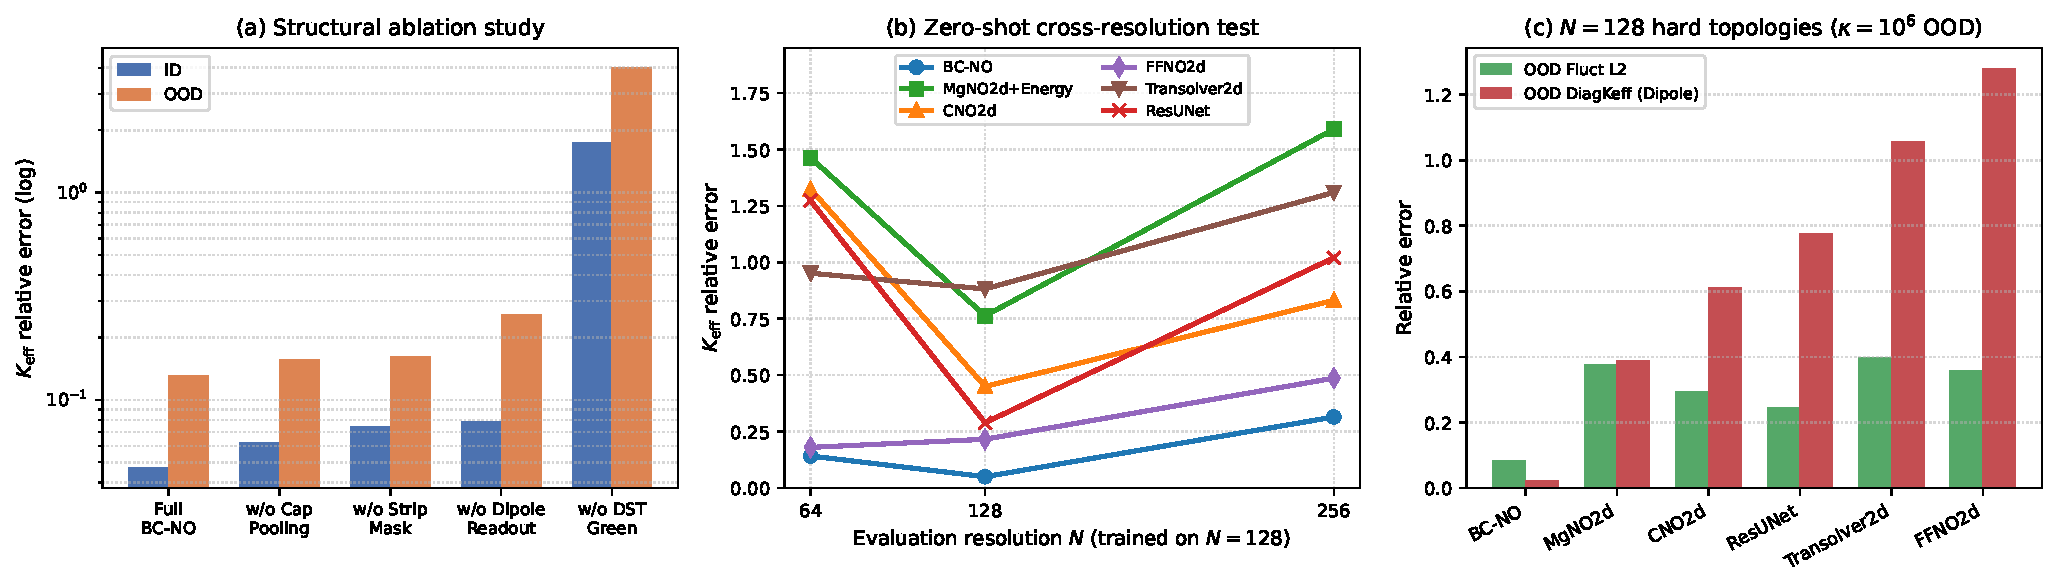
\includegraphics[width=\textwidth]{fig3_ablation_crossres_hard.pdf}
  \caption{(a) Structural ablations on $N=128$ \texttt{fiber\_columns}. (b) Zero-shot cross-resolution evaluation ($N=64, 256$) of models trained exclusively at $N=128$. (c) $N=128$ hard topologies at $\kappa=10^6$ OOD.}
  \label{fig:ablation_crossres}
\end{figure}

Table~\ref{tab:scale_ablation} (right, an independent 75-epoch 3-seed run) and Fig.~\ref{fig:ablation_crossres}(a) isolate each module:
(i) replacing the $\mathrm{DST}$-I Green operator $G_0$ with direct local convolutional prediction of $v_\theta$ (\texttt{w/o DST Green}) raises errors to $1.753$ ID / $3.997$ OOD;
(ii) disabling component capacitance pooling (\texttt{w/o Cap Pooling}) degrades OOD fluctuation $L^2$ by $58\%$ ($0.220 \to 0.348$);
(iii) removing the one-cell strip mask (\texttt{w/o Strip Mask}) increases ID $\Keff$ error by $57\%$ ($0.047 \to 0.074$) and ID fluctuation error by $40\%$;
(iv) replacing~\eqref{eq:dipole_id} with conservative fluxes (\texttt{w/o Dipole Readout}) nearly doubles OOD $\Keff$ error ($0.131 \to 0.257$).

On zero-shot cross-resolution inference (models trained solely at $N=128$, tested at $N=64, 256$; Fig.~\ref{fig:ablation_crossres}(b)), BC-NO maintains the lowest $\Keff$ error ($0.142$ at $N=64$, $0.050$ at $128$, $0.315$ at $256$, vs.\ $0.461$--$1.881$ at $N=64$ and $0.49$--$1.91$ at $N=256$ for naive baselines), yet exhibits a $6\times$ error increase from $N=128$ to $256$. Exp.~5b (Fig.~\ref{fig:rigor_v5}(a), 3 seeds, zero $N=256$ training) compares single-resolution $N=128$ training against multi-resolution $N\in\{64,128\}$ training while tracking the interface density error $\norm{(\sigma_\theta - \sigma)\mathbf{1}_{\partial I}}_2 / \norm{\sigma\mathbf{1}_{\partial I}}_2$. Under $80$-epoch single-resolution $N=128$ training, BC-NO yields $\Keff$ errors of $0.108\pm 0.012$ ($N=64$), $0.037\pm 0.003$ ($N=128$), and $0.149\pm 0.050$ ($N=256$; $0.087$ diagonal), while $\sigma_{\partial I}$ error rises from $0.088$ ($128$) to $0.133$ ($64$) and $0.162$ ($256$). Multi-resolution $N\in\{64,128\}$ training reduces $N=64$ $\sigma_{\partial I}$ error ($0.133\to 0.106$) and lowers $N=256$ $\Keff$ error to $0.129\pm 0.043$ ($0.070$ diagonal; whereas multi-resolution \texttt{FFNO2d} reaches $0.793\pm 0.086$), yet $N=256$ $\sigma_{\partial I}$ error remains $0.168$. Thus, although the definition $\sigma = h L_0 v$ is $1/h$-scaled, the learned fixed-pixel convolutional block $\mathcal{B}_\theta$ experiences receptive-field and sub-cell strip shift when extrapolating to finer grids.

On \textbf{same-hardware} 4-thread Apple M3 CPU timing across $N \in \{64, 128, 256, 512\}$, sparse LU scales as $7.41 \to 28.73 \to 181.80 \to 1{,}266.35\text{ ms}$ per sample, while BC-NO on the identical CPU scales as $5.76 \to 33.43 \to 129.19 \to 605.99\text{ ms}$ ($0.86\times$ at $N=128$---slower than sparse LU---then $1.41\times$ at $256$ and $2.09\times$ at $N=512$). Matched-accuracy early-stopping of Willot CG-FFT on the same GPU (Sec.~\ref{sec:setup}) reaches the $5\%$--$30\%$ $\Keff$ error band in $3$--$7$ iterations ($\approx 11$--$13\text{ ms}$). In the two-scale setting the relevant cost is the constitutive map evaluated at every macroscopic quadrature point; BC-NO supplies that map in a fixed number of Green layers without an outer Krylov loop.

\subsection{Periodic BCs, Classical Willot CG-FFT, and 2D Linear Elasticity (Exp.~7 \& Exp.~9)}\label{sec:exp_pbc_elas}

\begin{figure}[t]
  \centering
  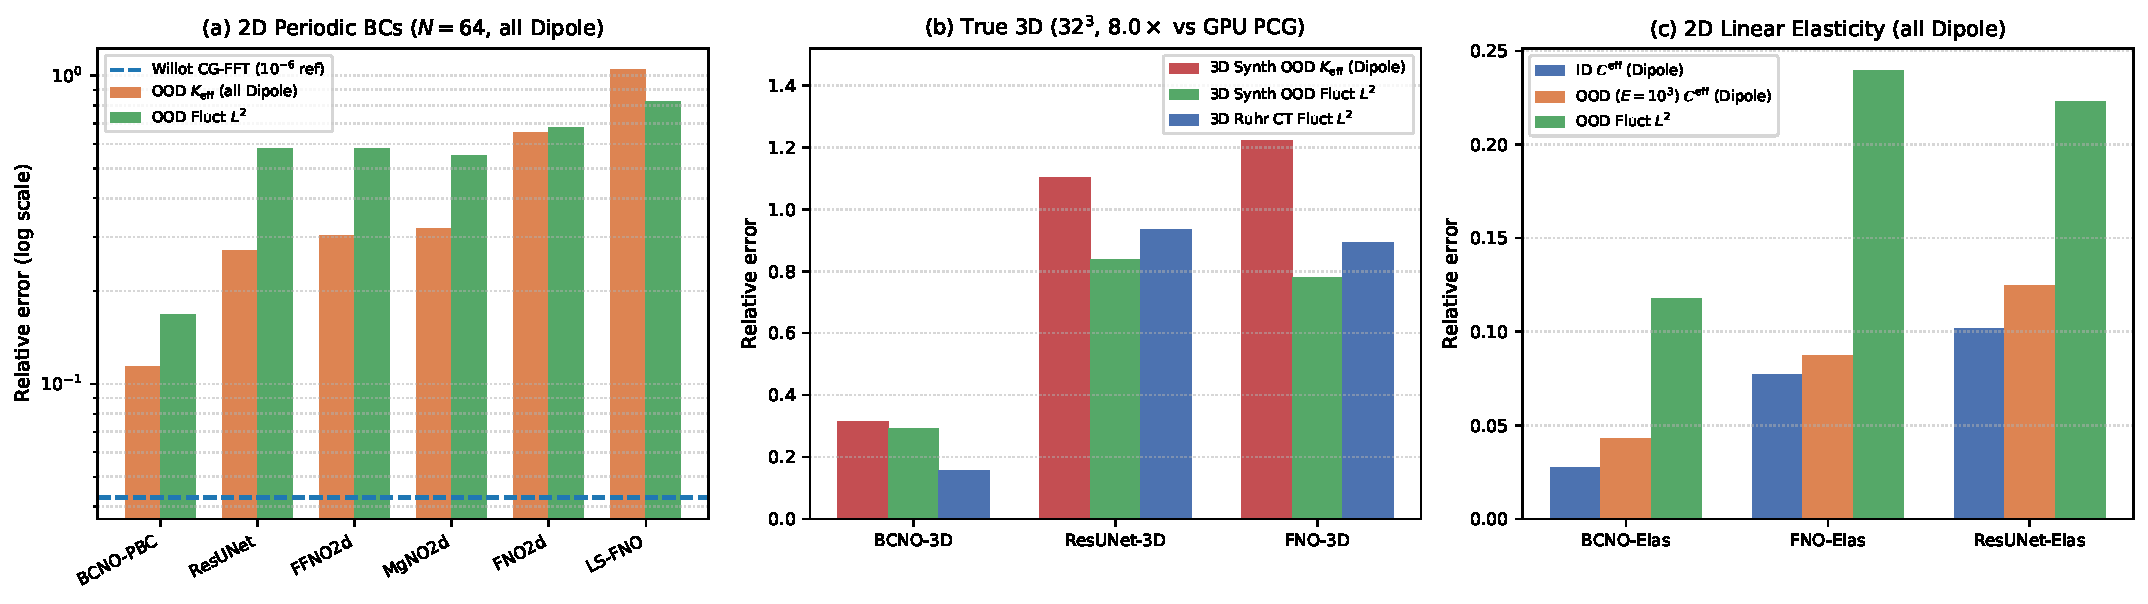
\includegraphics[width=\textwidth]{fig5_pbc_3d_elasticity.pdf}
  \caption{Generality across PDE classes and dimensions (3 seeds, all models using dipole readout). (a) 2D periodic boundary conditions ($N=64$) with classical Willot CG-FFT ($\mathrm{tol}=10^{-6}$) reference. (b) True 3D ($32^3$) with non-collapsed baselines and same-GPU PCG speedup ($8.0\times$). (c) 2D periodic Q1 linear elasticity ($E_1/E_0 = 10^3$ OOD).}
  \label{fig:pbc_3d_elas}
\end{figure}

\begin{table}[t]
\centering
\caption{Exp.~7: 2D Periodic BCs ($N=64$, wrapped inclusions) vs.\ classical Willot CG-FFT and \texttt{LS-FNO}; Exp.~9: 2D Periodic Q1 Linear Elasticity ($E_1/E_0=10^3$ OOD); 3 seeds, mean $\pm$ std. All learned models use dipole readout (Dip, primary) alongside naive readout.}
\label{tab:pbc_elas}
\resizebox{\textwidth}{!}{%
\begin{tabular}{@{}llccccc@{}}
\toprule
Problem & Model & ID Tensor Dip & ID Fluct $L^2$ & OOD Tensor Dip & OOD Tensor Naive & OOD Fluct $L^2$ \\
\midrule
\multirow{7}{*}{2D Periodic ($64^2$)}
 & Willot CG-FFT ($\mathrm{tol}=10^{-6}$) & 0.029 ($30$ it, $4.17\text{ ms}$) & --- & 0.043 ($45$ it, $2.20\text{ ms}$) & --- & --- \\
 & \textbf{BCNO-PBC} & \textbf{0.027}$\pm$0.001 & \textbf{0.086}$\pm$0.003 & \textbf{0.114}$\pm$0.002 & \textbf{0.332}$\pm$0.035 & \textbf{0.168}$\pm$0.005 \\
 & ResUNet & 0.138$\pm$0.009 & 0.552$\pm$0.007 & 0.270$\pm$0.011 & 1.361$\pm$0.110 & 0.582$\pm$0.001 \\
 & FFNO2d & 0.124$\pm$0.012 & 0.547$\pm$0.021 & 0.304$\pm$0.029 & 1.837$\pm$0.380 & 0.582$\pm$0.027 \\
 & MgNO2d & 0.137$\pm$0.004 & 0.523$\pm$0.007 & 0.319$\pm$0.024 & 2.020$\pm$0.052 & 0.553$\pm$0.017 \\
 & FNO2d & 0.297$\pm$0.048 & 0.644$\pm$0.052 & 0.653$\pm$0.108 & 6.946$\pm$1.743 & 0.678$\pm$0.053 \\
 & LS-FNO & 0.505$\pm$0.001 & 0.823$\pm$0.002 & 1.046$\pm$0.002 & 13.566$\pm$0.039 & 0.824$\pm$0.001 \\
\midrule
\multirow{3}{*}{2D Elasticity ($\Ceff$)}
 & \textbf{BCNO-Elas} & \textbf{0.027}$\pm$0.000 & \textbf{0.069}$\pm$0.001 & \textbf{0.043}$\pm$0.000 & \textbf{0.476}$\pm$0.083 & \textbf{0.118}$\pm$0.003 \\
 & FNO-Elas & 0.077$\pm$0.006 & 0.195$\pm$0.005 & 0.088$\pm$0.003 & 0.975$\pm$0.219 & 0.239$\pm$0.006 \\
 & ResUNet-Elas & 0.102$\pm$0.004 & 0.180$\pm$0.001 & 0.125$\pm$0.005 & 1.611$\pm$0.513 & 0.223$\pm$0.005 \\
\bottomrule
\end{tabular}}
\end{table}

Table~\ref{tab:pbc_elas} and Fig.~\ref{fig:pbc_3d_elas}(a,c) evaluate the periodic torus and vector solid-mechanics extensions under unified dipole evaluation. On 2D PBC ($N=64$), classical Willot rotated-grid CG-FFT ($\mathrm{tol}=10^{-6}$) converges in $30$--$45$ GPU iterations ($4.17\text{ ms}$ ID, $2.20\text{ ms}$ OOD). Its $2.9\%$ ID / $4.3\%$ OOD discrepancy against our harmonic-face FVM reference measures the difference between rotated-grid FFT and node-centered FVM discretizations. Among single-pass neural surrogates, \texttt{BCNO-PBC} attains $2.7\%$ ID and $11.4\%$ OOD dipole error ($0.9\text{ ms}$), $2.4\times$ below the strongest learned baseline (ResUNet $0.270$; $9.2\times$ only vs.\ the weakest, \texttt{LS-FNO} $1.046$). On 2D periodic Q1 linear elasticity at $E_1/E_0 = 10^3$, \texttt{BCNO-Elas} attains $2.7\%$ ID and $4.3\%$ OOD $\Ceff$ error ($2.0\times$ below FNO-Elas $0.088$).

\subsection{True 3D Homogenization ($32^3, 64^3$) and Real Micro-CT Volumes (Exp.~6, 8, 12)}\label{sec:exp_3d_ct}

\begin{figure}[t]
  \centering
  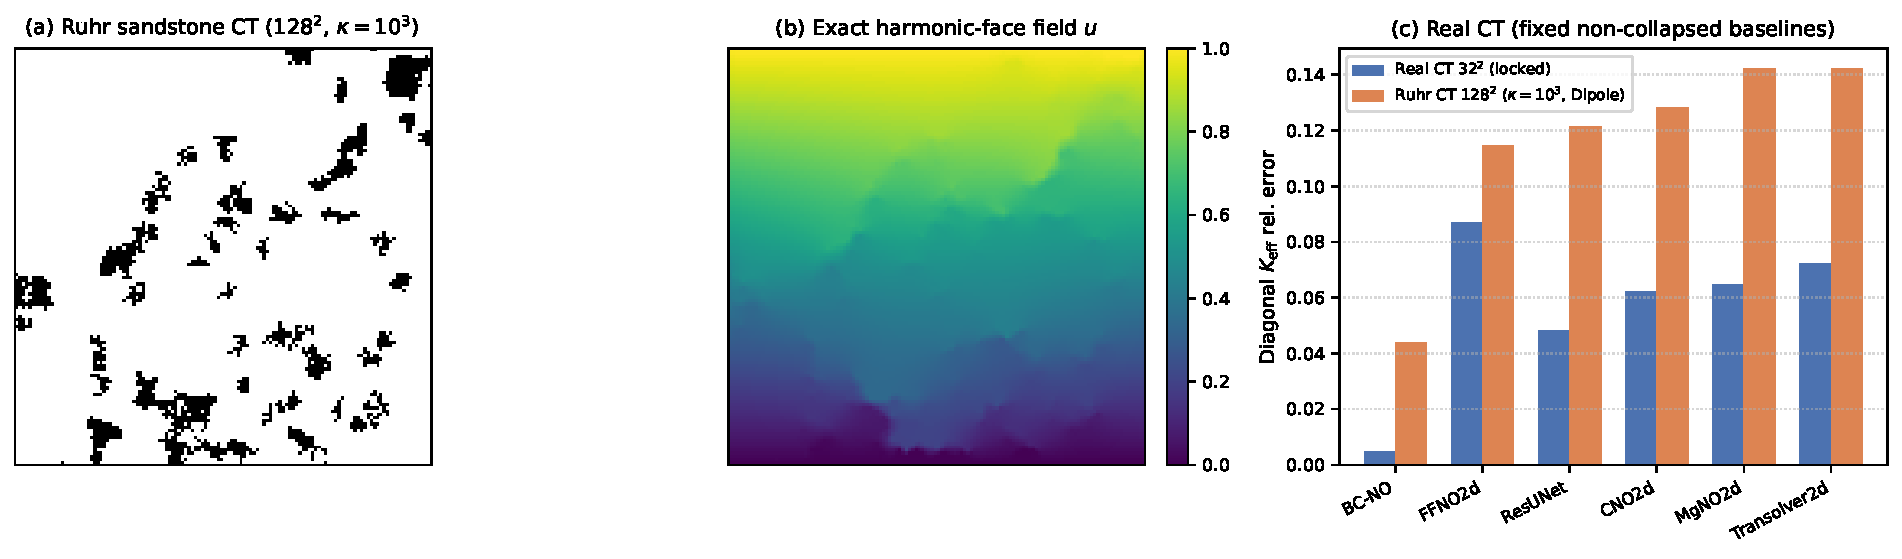
\includegraphics[width=\textwidth]{fig4_real_ct_microstructures.pdf}
  \caption{Real micro-CT validation. (a) $128^2$ Ruhr sandstone slice ($\kappa_{\mathrm{mineral}} = 10^3$, $\kappa_{\mathrm{pore}} = 1$). (b) Exact harmonic-face potential $u$. (c) Diagonal $\Keff$ error across $32^2$ multi-mineral locked test and $128^2$ Ruhr sandstone using non-collapsed baselines (all Dipole on $128^2$).}
  \label{fig:real_ct}
\end{figure}

\begin{table}[t]
\centering
\caption{True 3D RVE benchmarks ($32^3$ 3 seeds, $64^3$ 1 seed) and real micro-CT datasets ($32^2$ locked test, $128^2$, $32^3$, $64^3$ Ruhr sandstone at $\kappa=10^3$), using non-collapsed re-trained baselines and unified Dipole (primary) / Naive readouts. Same-GPU Jacobi-PCG ($\mathrm{tol}=10^{-6}$): $32.2\text{ ms}$/axis at $32^3$ ($199$ iters); $71.9\text{ ms}$/axis at $64^3$ ($239$ iters).}
\label{tab:3d_ct}
\resizebox{\textwidth}{!}{%
\begin{tabular}{@{}llcccccc@{}}
\toprule
Dataset & Model & Params & ID / Test Dip & OOD Dip & OOD Naive & Fluct $L^2$ (ID/OOD) & GPU ms \\
\midrule
\multirow{3}{*}{3D Synth ($32^3$)}
 & \textbf{BCNO-3D} & \textbf{56,889} & \textbf{0.162}$\pm$0.004 & \textbf{0.315}$\pm$0.006 & \textbf{1.097}$\pm$0.030 & \textbf{0.286} / \textbf{0.292} & 4.01 (batch: 2.18) \\
 & FNO-3D (fixed) & 1,640,925 & 0.342$\pm$0.026 & 1.223$\pm$0.061 & 2.975$\pm$0.305 & 0.655 / 0.780 & 1.99 \\
 & ResUNet-3D (fixed) & 252,501 & 0.371$\pm$0.046 & 1.102$\pm$0.029 & 3.409$\pm$0.294 & 0.735 / 0.838 & 2.55 \\
\midrule
\multirow{3}{*}{3D Synth ($64^3$)}
 & \textbf{BCNO-3D} & \textbf{56,889} & \textbf{0.073} & \textbf{0.110} & --- & \textbf{0.168} / \textbf{0.219} & 26.33 (batch: 13.93) \\
 & ResUNet-3D (fixed) & 252,501 & 0.171 & 0.432 & 3.591 & 0.605 / 0.642 & 18.78 \\
 & FNO-3D (fixed) & 1,640,925 & 0.369 & 0.981 & 4.777 & 0.615 / 0.668 & 12.06 \\
\midrule
\multirow{3}{*}{3D Ruhr CT ($32^3$)}
 & \textbf{BCNO-3D} & \textbf{56,889} & \textbf{0.007}$\pm$0.001 & --- & --- & \textbf{0.157}$\pm$0.022 & 2.23 \\
 & ResUNet-3D (fixed) & 252,501 & 0.088$\pm$0.004 & --- & --- & 0.934$\pm$0.005 & 2.90 \\
 & FNO-3D (fixed) & 1,640,925 & 0.101$\pm$0.002 & --- & --- & 0.893$\pm$0.025 & 1.98 \\
\midrule
\multirow{3}{*}{3D Ruhr CT ($64^3$)}
 & \textbf{BCNO-3D} & \textbf{56,889} & \textbf{0.001} & --- & --- & \textbf{0.107} & 13.25 \\
 & ResUNet-3D (fixed) & 252,501 & 0.039 & --- & --- & 0.887 & 19.12 \\
 & FNO-3D (fixed) & 1,640,925 & 0.045 & --- & --- & 0.873 & 12.02 \\
\midrule
\multirow{6}{*}{2D CT ($32^2$ / $128^2$)}
 & \textbf{BC-NO} & \textbf{90,380} & \textbf{0.005} / \textbf{0.044} & --- & --- & \textbf{0.063} / \textbf{0.245} & 0.94 \\
 & ResUNet (fixed) & 843,009 & 0.048 / 0.122 & --- & --- & 0.678 / 0.916 & 1.25 \\
 & CNO2d (fixed) & 168,417 & 0.062 / 0.128 & --- & --- & 0.766 / 0.933 & 1.94 \\
 & MgNO2d (fixed) & 897,505 & 0.065 / 0.142 & --- & --- & 0.739 / 0.996 & 4.59 \\
 & Transolver2d (fixed) & 213,825 & 0.072 / 0.142 & --- & --- & 0.702 / 0.982 & 9.72 \\
 & FFNO2d (fixed) & 1,164,769 & 0.087 / 0.115 & --- & --- & 0.656 / 0.783 & 5.39 \\
\bottomrule
\end{tabular}}
\end{table}

Table~\ref{tab:3d_ct}, Fig.~\ref{fig:real_ct}, and Figs.~\ref{fig:pbc_3d_elas}(b)--\ref{fig:rigor_v5}(c) report true 3D homogenization ($32^3, 64^3$) and real micro-CT benchmarks using our \textbf{non-collapsed} re-trained baselines and unified dipole readouts. After removing the $10^{-3}$ head bottleneck, external 2D/3D baselines learn genuine non-zero fluctuations ($0.656$--$0.766$ $L^2$ on $32^2$ CT; $0.605$--$0.838$ on 3D Synth; $0.873$--$0.934$ on 3D Ruhr CT). On $32^2$ locked multi-mineral CT slices, BC-NO achieves $0.5\%$ $\Keff$ error versus $4.8\%$--$8.7\%$ for fixed baselines; on $128^2$ Ruhr sandstone ($\kappa = 10^3$), $4.4\%$ dipole vs.\ $11.5\%$--$14.2\%$. In 3D synthetic cells, $32^3$ OOD is $0.315$ versus $1.102$ for the strongest baseline ($3.5\times$); at $64^3$ (1 seed) OOD is $0.110$ versus $0.432$ ($3.9\times$), with $0.1\%$ $\Keff$ on Ruhr CT. On the same CUDA GPU, single-sample \texttt{BCNO-3D} runs in $4.01\text{ ms}$ / $26.33\text{ ms}$ at $32^3$/$64^3$, against $32.2$ / $71.9\text{ ms}$ per axis for Jacobi-PCG at $\mathrm{tol}=10^{-6}$ ($8.0\times$ / $2.7\times$).

\subsection{Nonlinear PDEs and Two-Scale Thermal/Elastic $\mathrm{FE}^2$ Deployment (Exp.~10, 13, 14)}\label{sec:exp_fe2_nl}

\begin{figure}[t]
  \centering
  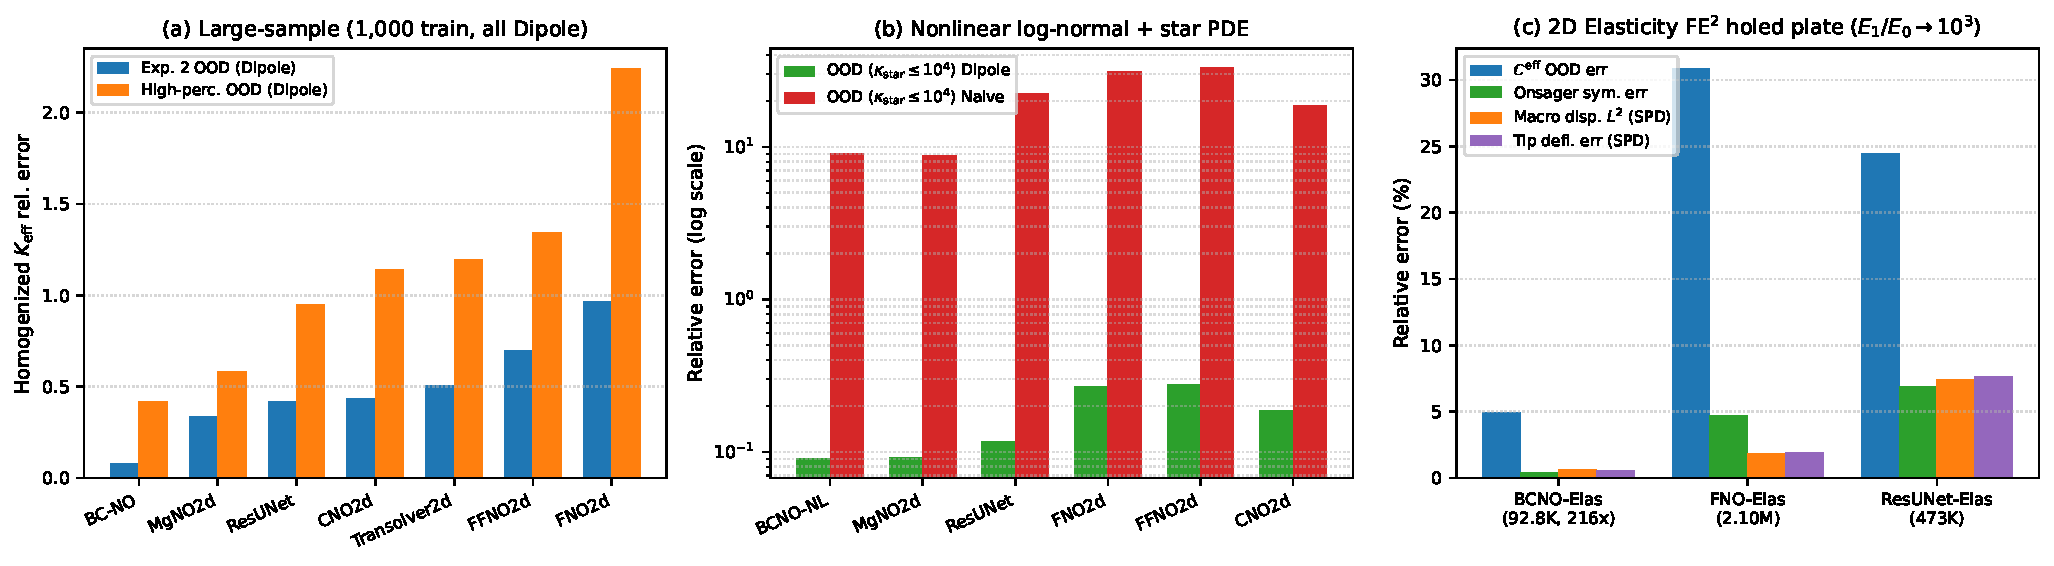
\includegraphics[width=\textwidth]{fig6_scale_3d64_nonlinear_fe2.pdf}
  \caption{(a) Exp.~11 large-sample $N=128$ ($1{,}000$ train, all models using dipole readout) on both Exp.~2 OOD and high-percolation OOD. (b) Exp.~13 nonlinear PDE $-\nabla\cdot(\kappa_0(x)(1+3u^2)\nabla u)=0$ on continuous log-normal matrices with sharp star inclusions. (c) Exp.~14 2D Q1 linear-elasticity $\mathrm{FE}^2$ holed composite cantilever ($184$ active RVEs, $E_1/E_0 \to 10^3$ OOD).}
  \label{fig:scale_fe2_nl}
\end{figure}

\begin{figure}[t]
  \centering
  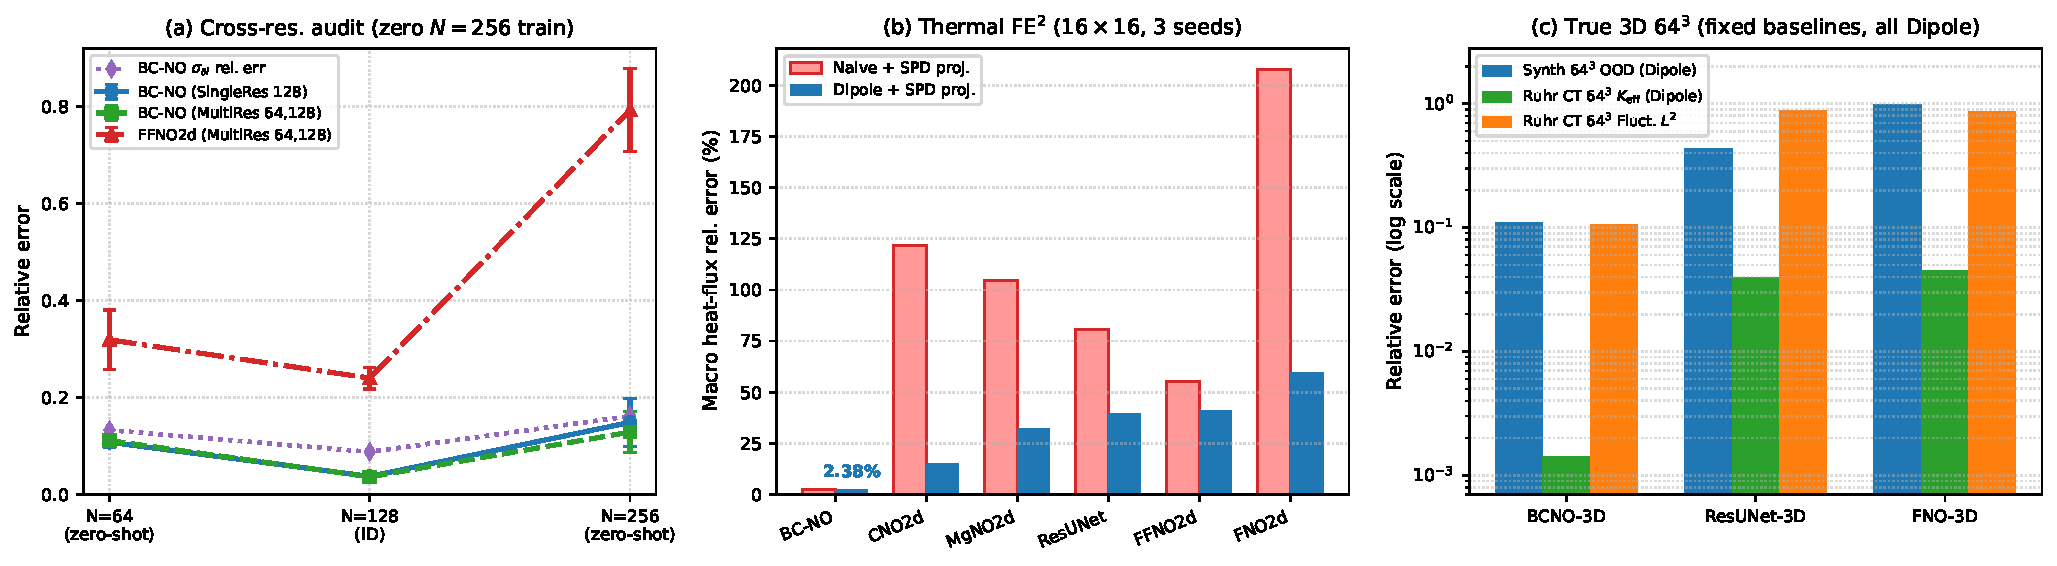
\includegraphics[width=\textwidth]{fig7_elasticity_fe2_rigor.pdf}
  \caption{(a) Exp.~5b controlled cross-resolution audit ($N=64, 128, 256$ with zero $N=256$ training, 3 seeds) including interface density error $\sigma_{\partial I}$. (b) Exp.~10 unified 3-seed thermal $\mathrm{FE}^2$ ($16\times 16$) macroscopic heat-flux error comparing Naive+SPD against Dipole+SPD across all models. (c) Exp.~12 true 3D $64^3$ composites and Ruhr sandstone CT using non-collapsed baselines and unified dipole readout.}
  \label{fig:rigor_v5}
\end{figure}

\begin{table}[t]
\centering
\caption{Exp.~10: Unified 3-seed OOD constitutive audit and $16\times 16$ thermal $\mathrm{FE}^2$ plate ($35.29\text{ s}$ CPU exact micro-solve time, comparing Raw, SPD-projected, and Dipole+SPD baselines); Exp.~13: nonlinear log-normal star PDE ($400$ train / $100$ ID / $100$ OOD).}
\label{tab:fe2_nl}
\resizebox{\textwidth}{!}{%
\begin{tabular}{@{}lccccccc|ccc@{}}
\toprule
Model & \multicolumn{2}{c}{OOD Audit} & \multicolumn{5}{c|}{$16\times 16$ Thermal $\mathrm{FE}^2$ Plate (3 seeds)} & \multicolumn{3}{c}{Exp.~13: Nonlinear Log-Normal + Star} \\
\cmidrule(lr){2-3}\cmidrule(lr){4-8}\cmidrule(lr){9-11}
 & Sym & SPD & Raw $T$ / Flux & SPD $T$ & SPD Flux & Dip+SPD Flux & Speedup & ID Dip (Naive) & OOD Dip / Naive & OOD Fluct \\
\midrule
\textbf{BC-NO} & \textbf{0.025} & \textbf{1.00} & \textbf{0.0251} / \textbf{0.0072} & \textbf{0.0236} & \textbf{0.0238} & \textbf{0.0238} & $35.8\times$ & \textbf{0.072} (0.379) & \textbf{0.091} / \textbf{9.10} & 0.171 \\
CNO2d & 0.122 & 0.98 & 0.0987 / 1.1728 & 0.1021 & 1.2168 & 0.1517 & $33.7\times$ & 0.144 (0.653) & 0.186 / 18.65 & 0.221 \\
MgNO2d & 0.118 & 0.90 & 0.0980 / 1.0321 & 0.1003 & 1.0478 & 0.3215 & $16.0\times$ & 0.087 (0.620) & 0.092 / 8.80 & 0.154 \\
ResUNet & 0.085 & 0.99 & 0.0849 / 0.7778 & 0.0862 & 0.8070 & 0.3957 & $50.6\times$ & 0.075 (0.536) & 0.117 / 22.49 & \textbf{0.149} \\
FFNO2d & 0.114 & 0.88 & 0.0974 / 0.4044 & 0.0915 & 0.5529 & 0.4095 & $11.9\times$ & 0.187 (0.532) & 0.277 / 32.92 & 0.205 \\
FNO2d & 0.054 & 1.00 & 0.1504 / 2.0752 & 0.1502 & 2.0768 & 0.5963 & $58.3\times$ & 0.258 (1.393) & 0.269 / 31.32 & 0.252 \\
\bottomrule
\end{tabular}}
\end{table}

\begin{table}[t]
\centering
\caption{Exp.~14: 2D Q1 linear-elasticity two-scale $\mathrm{FE}^2$ holed composite cantilever ($184$ active $64^2$ periodic RVEs $\times 3$ strain modes, $130.79\text{ s}$ CPU reference solves, $E_1/E_0 \in [30, 1000]$ OOD, models trained solely on $E_1/E_0 \in [10, 200]$). All models use dipole stress readout~\eqref{eq:elas_dipole}.}
\label{tab:elas_fe2}
\resizebox{\textwidth}{!}{%
\begin{tabular}{@{}lccccccccc@{}}
\toprule
Model & Params & Micro Infer (Speedup) & $\Ceff$ OOD Err & Onsager Sym & $\mathrm{SPD}_{\mathrm{raw}}$ ($\lambda_{\min}^{\mathrm{raw}}$) & Macro $U$ (Raw / SPD) & Strain Energy (SPD) & Tip Defl.\ (SPD) \\
\midrule
\textbf{BCNO-Elas} & \textbf{92,812} & $0.605\text{ s}$ ($216.1\times$) & \textbf{0.049} & \textbf{0.004} & \textbf{0.995} (\textbf{$-0.50$}) & \textbf{0.0352} / \textbf{0.0061} & \textbf{0.0074} & \textbf{0.0059} \\
FNO-Elas & 2,103,810 & $0.170\text{ s}$ ($770.2\times$) & 0.308 & 0.047 & 0.984 ($-80.79$) & 0.0598 / 0.0183 & 0.0141 & 0.0193 \\
ResUNet-Elas & 473,442 & $0.176\text{ s}$ ($741.3\times$) & 0.244 & 0.069 & 0.984 ($-38.80$) & 0.1450 / 0.0744 & 0.0763 & 0.0766 \\
\bottomrule
\end{tabular}}
\end{table}

Tables~\ref{tab:fe2_nl}--\ref{tab:elas_fe2} and Figs.~\ref{fig:scale_fe2_nl}--\ref{fig:rigor_v5}(b) validate two-scale deployment at intermediate contrast ($\kappa\in[20,250]$, $E_1/E_0$ up to $10^3$). On OOD \texttt{fiber\_columns}, BC-NO achieves $0.025$ Onsager symmetry error with $100\%$ SPD and $99.0\%$ Voigt--Reuss compliance~\cite{hashin1962variational}. In the unified 3-seed $16\times 16$ thermal $\mathrm{FE}^2$ plate, CPU micro-solves take $35.29\text{ s}$ while GPU BC-NO inference takes $0.986\text{ s}$ ($35.8\times$ wall-clock; cross-hardware workflow comparison). BC-NO achieves $2.51\%$ raw temperature $L^2$ and $0.72\%$ raw heat-flux error. Because $1.3\%$ of near-percolating graded cells have slightly negative eigenvalues ($\mathrm{spd\_rate}=0.987$), we clip eigenvalues at the isotropic Reuss lower bound $\lambda_{\min}\ge 1.0$ (matrix conductivity), restoring $100\%$ coercivity: temperature $L^2$ falls to $2.36\%$ while boundary heat-flux error rises to $2.38\%$ because clipping increases outflow diffusivity. Even with dipole+SPD, baseline flux errors remain $15.2\%$--$59.6\%$.

On the $20\times 10$ elastic cantilever (Exp.~14), \texttt{BCNO-Elas} evaluates $552$ RVE modes in $0.605\text{ s}$ GPU vs.\ $130.79\text{ s}$ CPU FEM ($216\times$ wall-clock workflow comparison), with $4.9\%$ OOD $\Ceff$ error. Elastic SPD uses $\lambda_{\min}\ge 0.5$ (half the matrix Young modulus scale used in training nondimensionalization), repairing one marginal cell ($\lambda_{\min}=-0.50$). Macro displacement / tip errors are $0.61\%$ / $0.59\%$. On the nonlinear star PDE (Exp.~13), post-hoc dipole alone brings \texttt{MgNO2d} OOD error to $9.2\%$, matching \texttt{BCNO-NL} ($9.1\%$): here the gain is readout, not architecture; \texttt{BCNO-NL} retains a modest ID edge ($7.2\%$ vs.\ $7.5\%$--$25.8\%$).

\section{Limitations and Concluding Remarks}\label{sec:conclusion}

The present scope is as follows. Corollary~\ref{cor:stab} covers non-percolating inclusions; wall-to-wall laminates use conservative fluxes, with percolating OOD diagonal errors of $15.8\%$ on \texttt{wavy\_laminate} and $42.1\%$ on high-percolation fibers. Zero-shot refinement from $N=128$ to $256$ raises $\Keff$ error from $0.037$ to $0.149$. Continuously varying matrices use an interior-relaxed strip mask. The $32^3$ synthetic OOD error is $0.315$; the $64^3$ Ruhr CT case is single-seed. Exp.~1 trains on 8 shapes. Warm-start PCG iteration counts drop by $6\%$--$14\%$.

In summary, relocating virtual-work averaging to the inclusion interface removes $\kappa$ from readout weights and, with capacitance-constrained Green updates, yields compact surrogates whose remaining architectural OOD gains versus the strongest all-dipole baseline are $1.0\times$--$4.1\times$ across the reported regimes, with the main engineering value in the intermediate-contrast $\mathrm{FE}^2$ band.

\section*{Data and Code Availability}
An implementation of BC-NO, together with scripts and data generators to reproduce every theorem verification, benchmark table, and figure in this study, is available at \url{https://github.com/LTQ12/BC-NO}.

\section*{Acknowledgments}
This work was supported by the Aeronautical Science Foundation of China (Grant 2023L039068002), the Basic Research Program of Science and Technology of Shenzhen (Grant JCYJ20250604122930040), and the Fundamental Research Funds for the Central Universities (Grant 20720230042).

\section*{Declaration of Competing Interest}
The authors declare that they have no known competing financial interests or personal relationships that could have appeared to influence the work reported in this paper.

\bibliographystyle{elsarticle-num}
\bibliography{refs}

\end{document}
